%!TEX encoding = UTF-8 Unicode 

\newif\ifen\enfalse
% Language selector; must be on line 3
% Change to false to export Korean

\documentclass[11pt,slidestop,compress,mathserif,notheorems]{beamer}
\usetheme{CambridgeUS}
\setbeamercovered{transparent}
\usepackage[parfill]{parskip}
\usepackage{layout}
\usepackage{color}
\usepackage{amsmath,amssymb}
\usepackage{amsthm}
\usepackage{graphicx}
\usepackage{relsize}
\usepackage{kotex}
\usepackage{diagbox}
\usepackage{multirow}
\usepackage{hyperref}
\hyperbaseurl{}
\urlstyle{same}
\usepackage[ruled]{algorithm2e}
\newcommand{\lIfElse}[3]{\lIf{#1}{#2 \textbf{else}~#3}}
%\usepackage{bbold}
%\usepackage{kbordermatrix}
\usepackage{xcolor}
%\usepackage{cutwin}
\usepackage{tabularx}
%\usepackage{pgfplots}
%\usepgfplotslibrary{external} % Prevents memory overflow issues w pgfplots
%\tikzexternalize
%\setlength{\jot}{0pt}


\usepackage{stackengine}
\newcommand\xrowht[2][0]{\addstackgap[.5\dimexpr#2\relax]{\vphantom{#1}}}



\ifen
{
\newtheorem{theorem}{Theorem}
\newtheorem{lemma}{Lemma}
\newtheorem{corollary}{Corollary}
\newtheorem{conjecture}{Conjecture}
\theoremstyle{definition}
\newtheorem{definition}{Definition}
\newtheorem{assumption}{Assumption}
\newtheorem{proposition}{Proposition}
\newtheorem{example}{Example}
\newtheorem{problem}{Problem}
}
\else {
\newtheorem{theorem}{정리}
\newtheorem{lemma}{기본정리}
\newtheorem{corollary}{따름정리}
\newtheorem{conjecture}{추측}
\theoremstyle{definition}
\newtheorem{definition}{정의}
\newtheorem{assumption}{가정}
\newtheorem{proposition}{제의}
\newtheorem{example}{예}
\newtheorem{problem}{문제}
}
\fi

\ifen \else \renewcommand{\proofname}{증명\@} \fi

\DeclareMathOperator*{\argmin}{arg\,min}
\DeclareMathOperator*{\argmax}{arg\,max}
\DeclareMathOperator*{\expd}{exp.}
\DeclareMathOperator*{\BR}{BR}

\newcommand*{\vertbar}{\rule[-1ex]{0.5pt}{2.5ex}}
\newcommand*{\horzbar}{\rule[.5ex]{2.5ex}{0.5pt}}
\setcounter{MaxMatrixCols}{20}

\DeclareGraphicsExtensions{.pdf,.png,.jpg}
\def\pfbox{\,\lower0.9pt\vbox{\hrule \hbox{\vrule height 0.2
cm \hskip 0.2 cm \vrule height 0.2 cm}\hrule}\,}
\newcommand{\nimplies}{%
  \mathrel{{\ooalign{\hidewidth$\not\phantom{=}$\hidewidth\cr$\implies$}}}}





\ifen 
\title{The College Application Problem}
\author{Max Kapur and Sung-Pil Hong}
\institute{Seoul National University\\
Department of Industrial Engineering \\
Management Science/Optimization Lab}
\date{\today}
\else
\title[대학 지원 최적화 문제]{대학 지원 최적화 문제}
\author{Max Kapur \& 홍성필}
\institute{서울대학교\\
산업공학과 \\
경영과학/최적화 연구실}
\date{\today}
\fi


\beamertemplatenavigationsymbolsempty

\definecolor{teal}{HTML}{008080}
\definecolor{olivedrab}{HTML}{6b8e23}
\definecolor{crimson}{HTML}{b22222}
\definecolor{palettetertiary}{HTML}{4169E1}
\definecolor{beige}{HTML}{f5fffa}
\definecolor{azure}{HTML}{F5F5F5}
\definecolor{rebeccapurple}{HTML}{663399}

% Corrects color spacing issue in math mode
\makeatletter
\renewcommand*{\@textcolor}[3]{%
  \protect\leavevmode
  \begingroup
    \color#1{#2}#3%
  \endgroup
}
\makeatother


\setbeamercolor{normal text}{fg=black,bg=white}
\setbeamercolor{alerted text}{fg=red}
\setbeamercolor{example text}{fg=black}

\setbeamercolor{palette primary}{fg=black, bg=beige}
%%\setbeamercolor{palette secondary}{fg=black, bg=beige}
\setbeamercolor{palette tertiary}{fg=white, bg=palettetertiary}

\setbeamercolor{frametitle}{fg=black, bg=azure}
\setbeamercolor{title}{fg=black, bg=azure}

\setbeamertemplate{items}[square]
\setbeamercolor*{item}{fg=palettetertiary}
%\beamertemplateshadingbackground{white}{white}
%\setbeamertemplate{caption}[numbered]
\setbeamertemplate{headline}{}



 \setbeamertemplate{caption}[numbered]
\setbeamertemplate{footline} {
  \leavevmode%
  \hbox{%
  \begin{beamercolorbox}[wd=.25\paperwidth,ht=2.65ex,dp=1.2ex,left]{author in head/foot}%
  \hspace*{1.5ex}\insertshortauthor
  \end{beamercolorbox}%
  \begin{beamercolorbox}[wd=.27\paperwidth,ht=2.65ex,dp=1.2ex,left]{date in head/foot}%
  \hspace*{1ex}
    \ifnum \theframenumber=1{}
    \else \insertshorttitle%~\textbar~\insertsectionhead
    \fi
     \end{beamercolorbox}%
  \begin{beamercolorbox}[wd=.23\paperwidth,ht=2.65ex,dp=1.2ex,right]{date in head/foot}%
    \ifnum \theframenumber=1{}
    \else \insertsectionhead
    \fi
  \hspace*{2ex}
     \end{beamercolorbox}%
       \begin{beamercolorbox}[wd=.15\paperwidth,ht=2.65ex,dp=1.2ex,left]{author in head/foot}%
  \hspace*{1.5ex}\insertdate
  \end{beamercolorbox}%
  \begin{beamercolorbox}[wd=.1\paperwidth,ht=2.65ex,dp=1.2ex,right]{author in head/foot}%
    \insertframenumber{} / \inserttotalframenumber
    \hspace*{1.5ex}
  \end{beamercolorbox}
}%
  \vskip0pt%
}

\overfullrule=0pt
\newcounter{usec}[section]

\makeatletter
\newcommand{\rmnum}[1]{\romannumeral #1}
\newcommand{\Rmnum}[1]{\expandafter\@slowromancap\romannumeral #1@}
\makeatother
\setbeamertemplate{theorems}[numbered]





\begin{document}


\begin{frame}
\titlepage
\end{frame}





\ifen \section{Introduction} \else \section{서론} \fi







\ifen {
\begin{frame}{Introduction}
The optimal college application problem is a \textbf{novel combinatorial optimization problem}.

\textbf{Maximize the expected maximum} of a portfolio of random variables subject to a budget constraint.

Today's agenda:
\begin{itemize}
\item \textbf{Formulate} college application as an optimization problem.
\item The \textbf{status quo} in admissions consulting, and why common heuristics fall short.
\item Our theoretical results, \textbf{solution algorithms}, and Julia implementation.
\end{itemize}

\textbf{Proofs and additional results} in our arXiv paper (Kapur and Hong 2022). 
\end{frame}
} \else {
\begin{frame}{서론}
대학 지원 최적화 문제란 \textbf{새로운 조합 최적화 문제}이다.

예산 제약 조선 하에서, 다수 확률 변수로 이뤄진 포트폴리오의 \textbf{기대 최댓값을 최대화한다}.

발표 요약:
\begin{itemize}
\item 대학 지원 전략을 최적화 문제로 \textbf{모형화}.
\item \textbf{현재 상황}: 입학 컨설팅 산업에서 흔히 사용하는 휴리스틱의 부족함.
\item 본 연구가 제시하는 \textbf{이론적 결과, 해법, 알고리즘 구현}.
\end{itemize}
\end{frame}
} \fi









\ifen {
\begin{frame}{Methodological orientation}
College application spans several areas of combinatorial optimization:

\begin{itemize}
\item Investment with uncertain payoff, search for the efficient frontier recall \textbf{portfolio allocation} models. 
\item Generalizes the \textbf{knapsack problem}: Integral packing constraint, NP-completeness.
\item Objective is a \textbf{submodular set function}, but approximation results suggest college application is a relatively easy instance. 
\end{itemize}
\end{frame}
} \else {
\begin{frame}{방법론적 지향}
대학 지원 전략은 조합 최적화 중 여러 분야를 걸친다.

\begin{itemize}
\item 불확실한 성과, 효율적 투자선이 존재하는 일종의 \textbf{포트폴리오 배분} 모형. 
\item \textbf{배낭 문제}의 일반화: 정수 패킹 제약식, NP-completeness.
\item 목적함수는 \textbf{submodular 집합 함수}이며, 근사 해법 결과에 따라 대학 지원 문제가 submodular 최적화의 비교적 쉬운 인스턴스로 해석할 수 있다.
\end{itemize}
\end{frame}

} \fi







\ifen \section{Model} \else \section{모형} \fi

\ifen {
\begin{frame}[plain]
  \vfill
\begin{center}
~
\begin{beamercolorbox}[wd=.5\textwidth,sep=8pt,center,shadow=false,rounded=true]{section in head/foot}
    \usebeamerfont{title} \insertsectionhead
  \end{beamercolorbox}
~
\end{center}
\end{frame}
} \else {
\begin{frame}[plain]
  \vfill
\begin{center}
~
\begin{beamercolorbox}[wd=.5\textwidth,sep=8pt,center,shadow=false,rounded=true]{section in head/foot}
    \usebeamerfont{title} \insertsectionhead
  \end{beamercolorbox}
~
\end{center}
\end{frame}
} \fi












\ifen {
\begin{frame}{The admissions process}
Consider a \textbf{single student's} college application decision.

Market contains $m$ \textbf{schools}, indexed by $\mathcal{C} = \{ 1\dots m\}$. School $j$ is named $c_j$.

Given a student's academic records, test scores, and demographic information, we can estimate her \textbf{admissions probability} $f_j$ at each school.

Let the \textbf{random variable} $Z_j \sim \operatorname{Bernoulli}(f_j) = 1$ if student is admitted, $0$ otherwise. Assume independent.

Let $\mathcal{X} \subseteq \mathcal{C}$ denote the set of schools, or \textbf{application portfolio}, to which a student applies.

Application fees, time to write essays, and/or legal limits \textbf{constrain} applicant behavior. We consider a single knapsack constraint $\sum_{j\in \mathcal{X}} g_j \leq H$ where $g_j$ is called $c_j$'s \textbf{application cost}. 
\end{frame}
} \else {
\begin{frame}{입학 과정}
단 \textbf{한 학생}의 의사결정에 집중하자.

시장은 $m$개의 \textbf{대학교}를 포함하며, 그의 지표 집합은 $\mathcal{C} = \{ 1\dots m\}$. $j$번째 학교의 이름은 $c_j$.

학생의 내신, 수능 점수, 기본 정보가 주어지면 각 학교의 \textbf{합격 확률} $f_j$를 추정할 수 있다.

\textbf{확률 변수} $Z_j \sim \operatorname{Bernoulli}(f_j)$는 학생이 합격하면 $1$, 아니면 $0$이다. 독립하다고 가정.

학생이 지원하는 학교의 집합 $\mathcal{X} \subseteq \mathcal{C}$를 \textbf{지원 포트폴리오}라고 부른다.

지원 수수료, 원서를 작성하는 시간, 또는 나라 정책에 따라 지원 행동이 \textbf{제한}된다. 본 논문은 단일 배낭 제약식 $\sum_{j\in \mathcal{X}} g_j \leq H$를 고려하며, 이때 $g_j$는 $c_j$의 \textbf{지원 비용}이라고 부른다. 
\end{frame}
} \fi






\ifen {
\begin{frame}{Utility model}
Let $t_j \geq 0$ denote the \textbf{utility} the student receives if she attends $c_j$. Wlog, $t_j \leq t_{j+1}$.

Let $t_0$ denote her utility if she doesn't get into college. Wlog, $t_0 =0$ (see paper).

The student's overall utility is the $t_j$-value associated with the \textbf{best} school she gets into:
\[\text{Utility} =\max\bigr\{t_0, \max\{t_j Z_j : j \in \mathcal{X}\}\bigr\}\]

When the student's application portfolio is $\mathcal{X}$, we refer to her expected utility as the portfolio's \textbf{valuation} $v(\mathcal{X})$. 
\end{frame}
} \else {
\begin{frame}{효용 모형}
$c_j$에 다니면 $t_j \geq 0$ 단위의 \textbf{효용}이 발생한다. Wlog, $t_j \leq t_{j+1}$.

어떤 대학에도 합격 안 하면 효용이 $t_0$이며, wlog $t_0 =0$임을 가정할 수 있다 (논문 참고).

학생의 전체 효용은 그가 합격하는 \textbf{가장 좋은} 학교의 $t_j$-값:
\[\text{효용} =\max\bigr\{t_0, \max\{t_j Z_j : j \in \mathcal{X}\}\bigr\}\]

지원 포트폴리오가 $\mathcal{X}$일 때, 기대 효용을 $\mathcal{X}$의 \textbf{가치}라고 부르며 $v(\mathcal{X})$처럼 표기한다.
\end{frame}
} \fi






\ifen {
\begin{frame}{Unpacking the portfolio valuation function}
To get $v(\mathcal{X})$ into a tractable form, let $p_j(\mathcal{X})$ denote the probability that the student \textbf{attends} $c_j$.

This happens if and only if she \textbf{applies} to $c_j$, is \textbf{admitted} to $c_j$, and is \textbf{not admitted} to any school she prefers to $c_j$:
\begin{align*}
p_j(\mathcal{X}) &= 
\begin{cases}
\displaystyle f_j  \prod_{\substack{i \in \mathcal{X}: \\ i > j}} (1 - f_{i}), \quad & j \in \{0\}\cup\mathcal{X}\\
0, \quad & \text{otherwise.}
\end{cases} 
\end{align*}

Therefore, 
\begin{align*}
v(\mathcal{X})
%&= \operatorname{E}\Bigl[\max\bigr\{t_0, \max\{t_j Z_j : j \in \mathcal{X}\}\bigr\}\Bigr] \\
&= \sum_{j=1}^m t_j p_j(\mathcal{X}) = \sum_{j\in \mathcal{X}} \Bigl( f_j t_j \prod_{\substack{i \in \mathcal{X}: \\ i > j}} (1 - f_{i}) \Bigr).  \label{closedformportfoliovaluationX}
\end{align*}

\end{frame}
} \else {
\begin{frame}{포트폴리오 가치의 함수 형태}
$v(\mathcal{X})$를 함수로 표현하기 위해, 학생이 $c_j$에 \textbf{진학하는} 확률을 $p_j(\mathcal{X})$라고 하자.

$c_j$에 진학하는 조견은 $c_j$에 \textbf{지원}하고, \textbf{합격}하고, $c_j$보다 선호하는 학교에 \textbf{합격하지 않는} 것이다:
\begin{align*}
p_j(\mathcal{X}) &= 
\begin{cases}
\displaystyle f_j  \prod_{\substack{i \in \mathcal{X}: \\ i > j}} (1 - f_{i}), \quad & j \in \{0\}\cup\mathcal{X}\\
0, \quad & \text{그러지 않은 경우.}
\end{cases} 
\end{align*}

따라서
\begin{align*}
v(\mathcal{X})
%&= \operatorname{E}\Bigl[\max\bigr\{t_0, \max\{t_j Z_j : j \in \mathcal{X}\}\bigr\}\Bigr] \\
&= \sum_{j=1}^m t_j p_j(\mathcal{X}) = \sum_{j\in \mathcal{X}} \Bigl( f_j t_j \prod_{\substack{i \in \mathcal{X}: \\ i > j}} (1 - f_{i}) \Bigr).  \label{closedformportfoliovaluationX}
\end{align*}

\end{frame}
} \fi







\ifen {
\begin{frame}{Problem statement}
\begin{problem}[The college application problem]
\vspace{-1em}
\begin{align*}
\begin{split}
\text{maximize}\quad &  v(\mathcal{X}) = \sum_{j\in \mathcal{X}} \Bigl(f_j t_j \prod_{\substack{i \in \mathcal{X}: \\ i > j}} (1 - f_{i}) \Bigr)\\
\text{subject to}\quad & \mathcal{X}\subseteq\mathcal{C}, \quad\sum_{j \in \mathcal{X}} g_j \leq H 
\end{split}
\end{align*}
\end{problem}

\begin{problem}[The college application problem, INLP form]% \label{integernlp}
\vspace{-1em}
\begin{align*}
\begin{split}
\text{maximize}\quad &  v(x) = \sum_{j=1}^m \Bigl(f_j t_j  x_j \prod_{i > j} (1 - f_{i} x_i) \Bigr)\\
\text{subject to}\quad & x_j \in \{0, 1\}, j \in \mathcal{C}; \quad \sum_{j=1}^m g_j x_j \leq H
\end{split}
\end{align*}
\end{problem}
\end{frame}
} \else {
\begin{frame}{문제 정의}
\begin{problem}[대학 지원 최적화 문제]
\vspace{-1em}
\begin{align*}
\begin{split}
\text{maximize}\quad &  v(\mathcal{X}) = \sum_{j\in \mathcal{X}} \Bigl(f_j t_j \prod_{\substack{i \in \mathcal{X}: \\ i > j}} (1 - f_{i}) \Bigr)\\
\text{subject to}\quad & \mathcal{X}\subseteq\mathcal{C}, \quad\sum_{j \in \mathcal{X}} g_j \leq H 
\end{split}
\end{align*}
\end{problem}

\begin{problem}[대학 지원 최적화 문제, 정수 비선형 계획 모형]% \label{integernlp}
\vspace{-1em}
\begin{align*}
\begin{split}
\text{maximize}\quad &  v(x) = \sum_{j=1}^m \Bigl(f_j t_j  x_j \prod_{i > j} (1 - f_{i} x_i) \Bigr)\\
\text{subject to}\quad & x_j \in \{0, 1\}, j \in \mathcal{C}; \quad \sum_{j=1}^m g_j x_j \leq H
\end{split}
\end{align*}
\end{problem}
\end{frame}
} \fi








\ifen \section{The status quo} \else \section{기존의 해법} \fi

\ifen {
\begin{frame}[plain]
  \vfill
\begin{center}
~
\begin{beamercolorbox}[wd=.5\textwidth,sep=8pt,center,shadow=false,rounded=true]{section in head/foot}
    \usebeamerfont{title} \insertsectionhead
  \end{beamercolorbox}
\end{center}
\end{frame}
} \else {
\begin{frame}[plain]
  \vfill
\begin{center}
~
\begin{beamercolorbox}[wd=.5\textwidth,sep=8pt,center,shadow=false,rounded=true]{section in head/foot}
    \usebeamerfont{title} \insertsectionhead
  \end{beamercolorbox}
\end{center}
\end{frame}
} \fi







\begin{frame}[plain]%{Safety, target, and reach schools}
\vfill 

\begin{center}
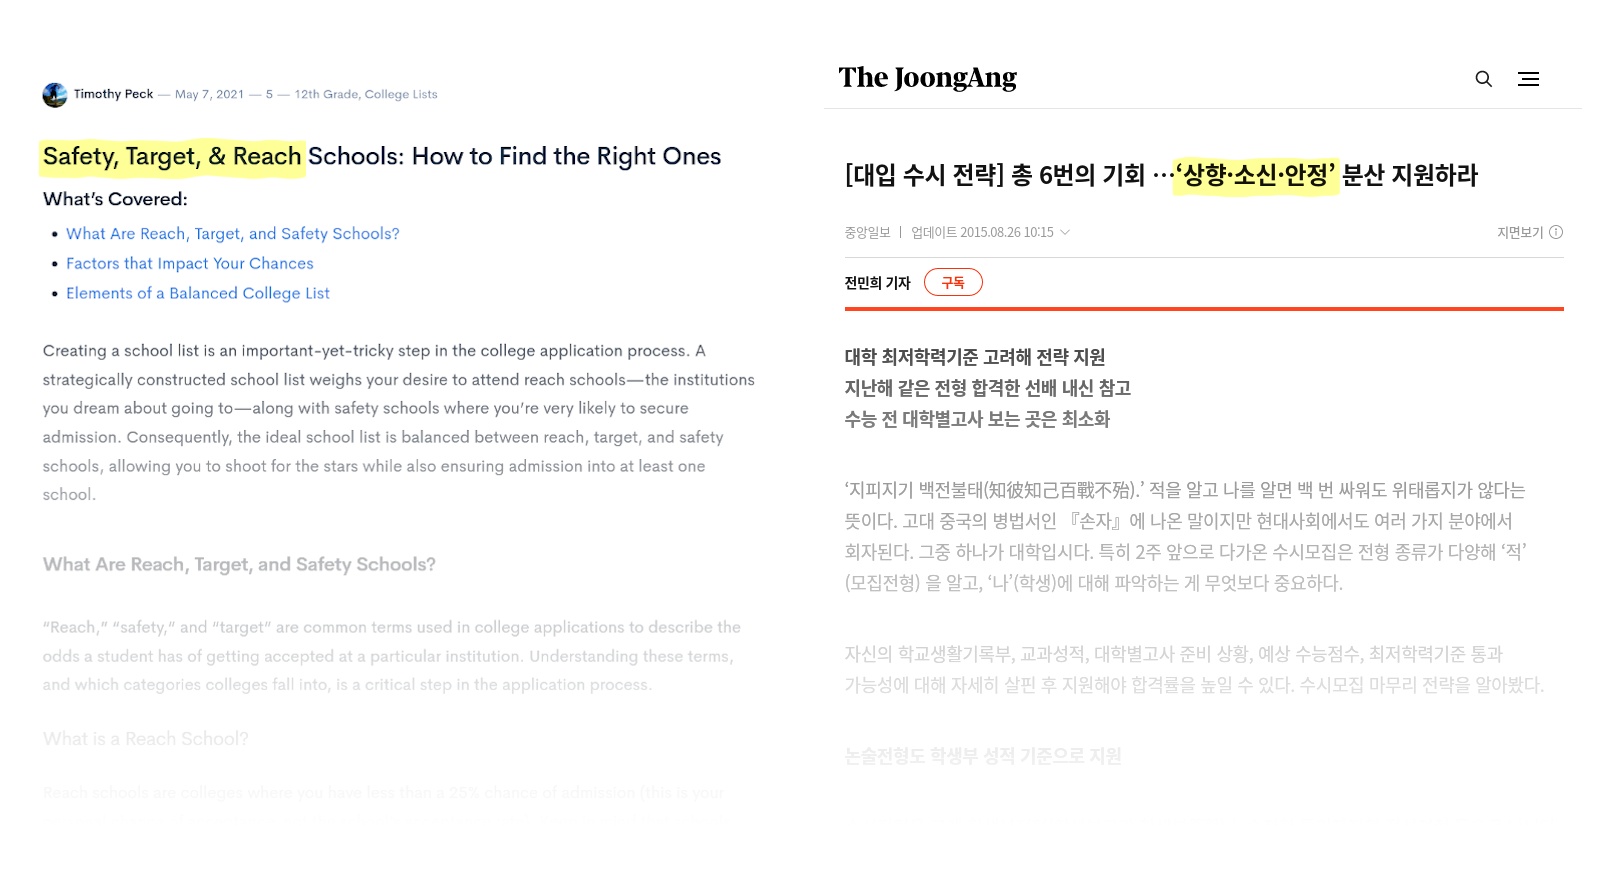
\includegraphics[width=\textwidth]{plots/news-both.png}

\ifen Can we trust the admissions consultant's advice?
\else 입학 컨설턴트의 조언, 믿을 만하는가? \fi
\end{center}

\end{frame}









\begin{frame}[plain]{}
\begin{center}
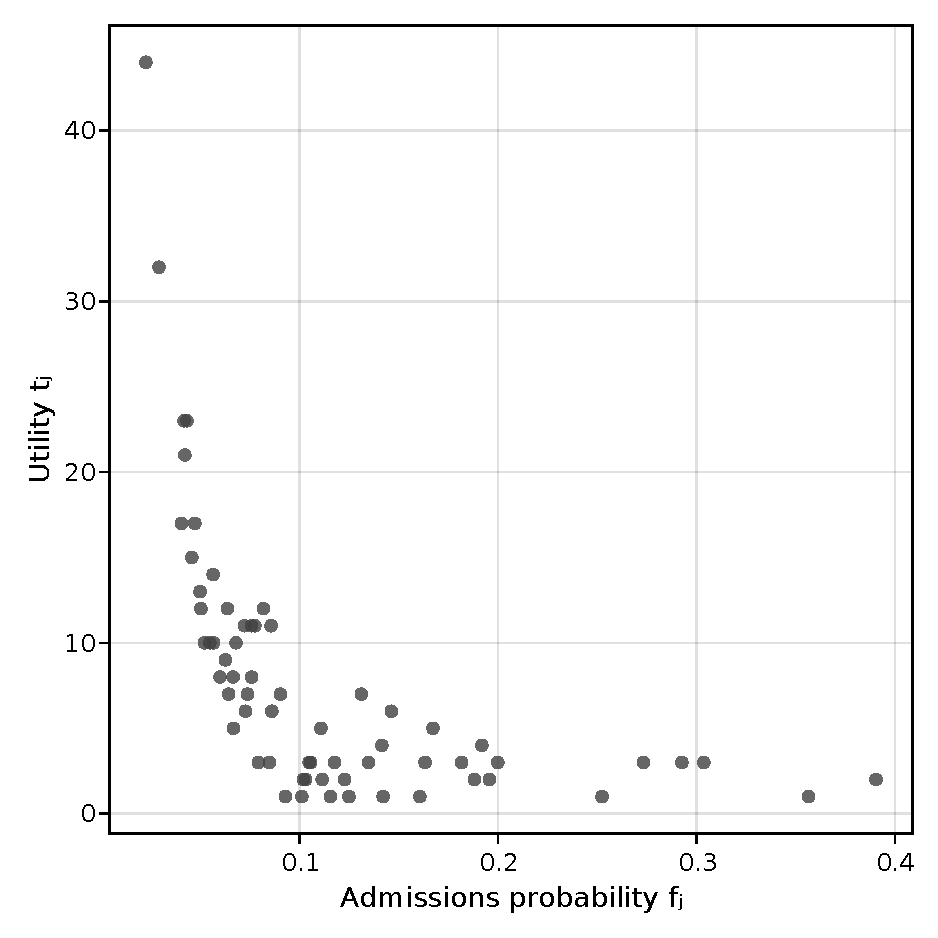
\includegraphics[height=\textheight]{plots/samplemarket.pdf}
\end{center}
\end{frame}





\begin{frame}[plain]{}
\begin{center}
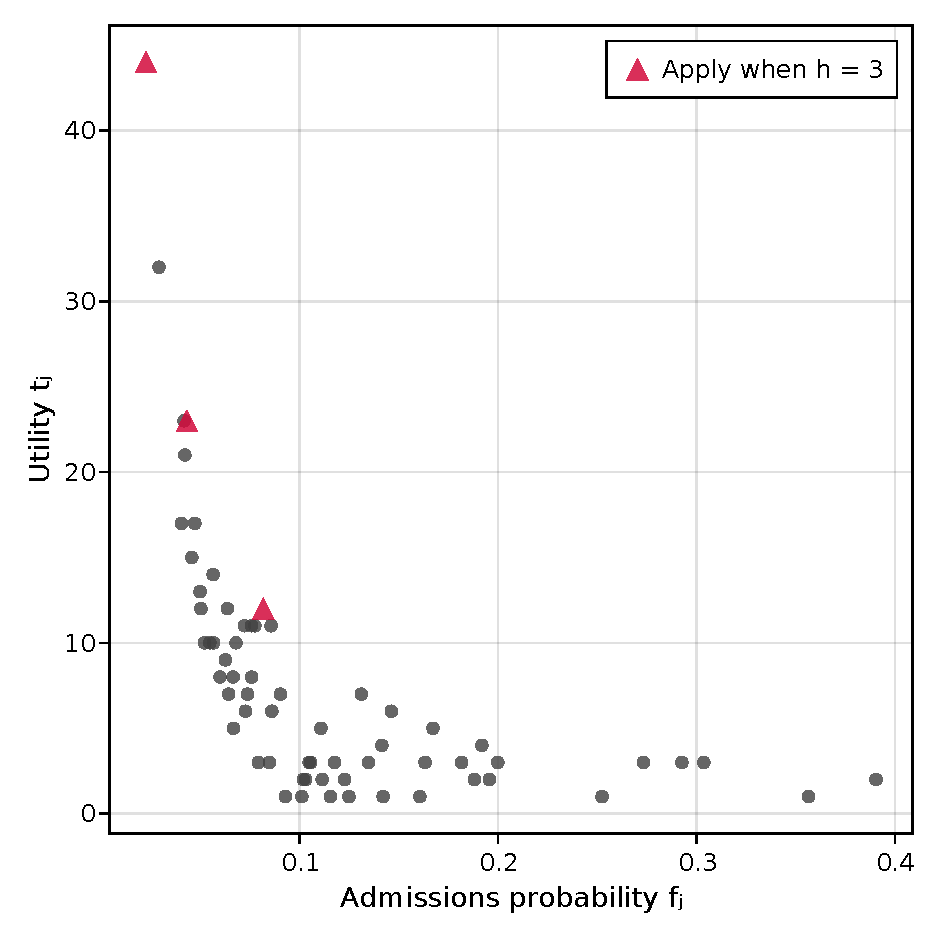
\includegraphics[height=\textheight]{plots/samplemarket-soln.pdf}
\end{center}
\end{frame}







\begin{frame}{Existing solutions}

In practice, most use \textbf{distributive heuristics} such as distributing applications evenly among attractive, selective ``reach schools'' and less-attractive ``safety schools.'' Turns out to be a \textbf{risk-averse} approach.

Another intuitive idea is the \textbf{linearization heuristic}. Since the expected utility associated with applying to $c_j$ (alone) is $f_j t_j$, solve the knapsack problem
\[\text{maximize}~~\sum_{j\in \mathcal{X}} f_j t_j \qquad \text{subject to}~~\sum_{j\in \mathcal{X}}g_j \leq H \]
as a surrogate. But this solution can be \textbf{arbitrarily bad}. 

Fu (2014) solved a similar problem by \textbf{enumeration}, which is intractable for $m \geq 20$ or so.

Our algorithms provide both \textbf{time and accuracy guarantees}. 

\end{frame}














\ifen \section{Our algorithms} \else \section{제시 알고리즘} \fi

\ifen {
\begin{frame}[plain]
  \vfill
\begin{center}
~
\begin{beamercolorbox}[wd=.5\textwidth,sep=8pt,center,shadow=false,rounded=true]{section in head/foot}
    \usebeamerfont{title} \insertsectionhead
  \end{beamercolorbox}
\end{center}
\end{frame}
} \else {
\begin{frame}[plain]
  \vfill
\begin{center}
~
\begin{beamercolorbox}[wd=.5\textwidth,sep=8pt,center,shadow=false,rounded=true]{section in head/foot}
    \usebeamerfont{title} \insertsectionhead
  \end{beamercolorbox}
\end{center}
\end{frame}
} \fi








\ifen {
\begin{frame}{Homogeneous costs: A polynomially solvable case}
We first consider the \textbf{special case} in which each $g_j = 1$ and $H$ is simply $h \leq m$, a limit on the number of schools you can apply to.

This case mirrors the main Korean admissions cycle, in which $h = 3, m= 202$. 

We show that when $\mathcal{X}_h$ is the optimal portfolio at $h$, $\mathcal{X}_{h} \subset \mathcal{X}_{h+1}$. This \textbf{nestedness property} implies the optimality of a \textbf{greedy algorithm} that adds schools one at a time, maximizing $v(\mathcal{X})$ at each addition.

Using a variable-elimination technique, we reduce the cost of computing $v(\mathcal{X})$ to amortized unit time, obtaining an $O(hm)$ algorithm. Our Julia implementation (Kapur 2022) solves an $m = 16384$ instance in 200 ms.

Strengthens the result of Fisher et al. (1978). 
\end{frame}
} \else {
\begin{frame}{다항 시간에 풀 수 있는 동일한 지원 비용의 경우}
먼저 모든 $g_j = 1$이며 $H$는 단순한 지원 개수 제한 $h \leq m$이 되는 \textbf{특수한 경우}를 고려하자. 

이것은 $h = 3, m= 202$인 한국 정시 입학 과정과 비슷한 상황이다.

지원 제한 $h$에 대응되는 최적 포트폴리오가 $\mathcal{X}_h$일 때, $\mathcal{X}_{h} \subset \mathcal{X}_{h+1}$을 증명할 수 있다. 이러한 \textbf{포함 사슬 관계 (nestedness)} 성질은 $v(\mathcal{X})$를 최대화하는 순서대로 학교를 하나씩 추가하는 \textbf{탐욕 해법}의 최적성을 의미한다.

변수 소거 기법은 개발하여 $v(\mathcal{X})$를 계산하는 시간을 환산 단위 시간을 줄임으로 $O(hm)$ 해법을 얻을 수 있다. 쥴리아 코드(Kapur 2022)를 사용하면 $m = 16384$인 인스턴스를 200 ms에 풀 수 있다.

Fisher et al. (1978)에 결과를 강화한다.
\end{frame}
} \fi










\ifen {
\begin{frame}{A small example}
College data and optimal application portfolios for a fictional market with $m=8$ schools.
\vspace{-1em}
\begin{center}
\begin{tabular}{r|lcccc}
\textbf{$j$} & \textbf{School $c_j$} & \textbf{Admit prob. $f_j$} & \textbf{Utility $t_j$} & \textbf{Priority} & \textbf{$v(\mathcal{X}_h)$} \\ \hline
\\[-.75em]
1 & Mercury University  & 0.39   & 200 & 4   & 230.0   \\
2 & Venus University    & 0.33   & 250 & 2   & 146.7  \\
3 & Mars University     & 0.24   & 300 & 6   & 281.5  \\
4 & Jupiter University  & 0.24   & 350 & 1   & \phantom{0}84.0  \\
5 & Saturn University   & 0.05   & 400 & 7   & 288.8  \\
6 & Uranus University   & 0.03   & 450 & 8   & 294.1  \\
7 & Neptune University  & 0.10   & 500 & 5   & 257.7  \\
8 & Pluto College       & 0.12   & 550 & 3   & 195.1      
\end{tabular}
\end{center}
By the nestedness property, the optimal portfolio when the application limit is $h$ consists of the $h$ schools having priority $h$ or less.

Valuation function appears on next slide. Always concave.
\end{frame}
} \else {
\begin{frame}{작은 예제}
$m=8$개의 학교로 이루어진 가상 입학 시장의 대학교 자료와 최적 지원 포트폴리오.
\begin{center}
\begin{tabular}{r|lcccc}
\textbf{지표 $j$} & \textbf{학교 $c_j$} & \textbf{합격 확률 $f_j$} & \textbf{효용 $t_j$}  & \textbf{지원 순위} & \textbf{$v(\mathcal{X}_h)$} \\ \hline
\\[-.75em]
1 & 수성대   & 0.39   & 200 & 4   & 230.0   \\
2 & 금성대   & 0.33   & 250 & 2   & 146.7  \\
3 & 화성대   & 0.24   & 300 & 6   & 281.5  \\
4 & 목성대   & 0.24   & 350 & 1   & \phantom{0}84.0  \\
5 & 토성대   & 0.05   & 400 & 7   & 288.8  \\
6 & 천왕성대  & 0.03   & 450 & 8   & 294.1  \\
7 & 해왕성대  & 0.10   & 500 & 5   & 257.7  \\
8 & 명왕성대  & 0.12   & 550 & 3   & 195.1      
\end{tabular}
\end{center}
포함 사슬 관계 성질에 따라, 지원 제한이 $h$일 때 최적 포트폴리오는 지원 순위가 $h$ 이하인 $h$개의 학교로 구성된다.
\end{frame}
} \fi












\begin{frame}[plain]
\begin{center}
 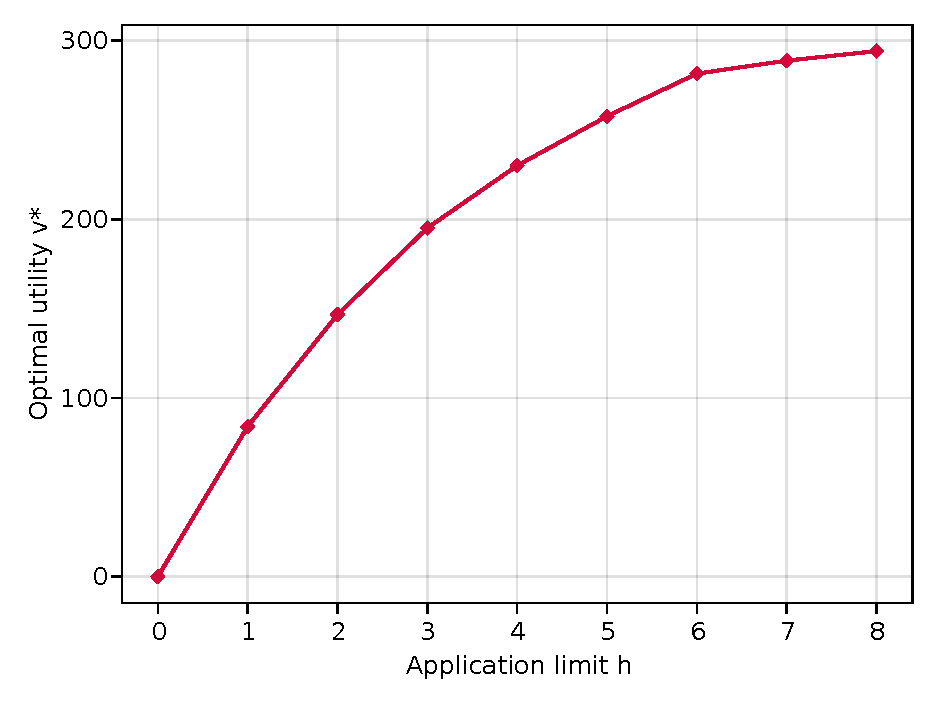
\includegraphics[height=\textheight]{./plots/h_v-example.pdf}
\end{center}
\end{frame}







\begin{frame}{Algorithms for the general problem}
The general problem is \textbf{NP-complete} (reduction from knapsack). We offer four algorithms:
\begin{itemize}
\item A linear relaxation and \textbf{branch-and-bound scheme}. Primarily of theoretical interest.

\item A \textbf{dynamic program based on total expenditures}. Exact solution in $O(Hm + m\log m)$ time (pseudopolynomial). Very fast for ``typical'' instances in which $g_j$ are small integers.

\item A different DP based on truncated portfolio valuations. $(1 - \varepsilon)$-optimal solution in $O(m^3 / \varepsilon)$ time: an \textbf{FPTAS}!
\item A \textbf{simulated annealing heuristic}. Fast, typically within 2\% of optimality.
\end{itemize}

Existence of FPTAS suggests college application is \textbf{a relatively easy instance of submodular maximization} (cf. Kulik et al. 2013).
\end{frame}










\ifen \section{Conclusion} \else \section{결론} \fi

\ifen {
\begin{frame}[plain]
  \vfill
\begin{center}
~
\begin{beamercolorbox}[wd=.5\textwidth,sep=8pt,center,shadow=false,rounded=true]{section in head/foot}
    \usebeamerfont{title} \insertsectionhead
  \end{beamercolorbox}
\end{center}
\end{frame}
} \else {
\begin{frame}[plain]
  \vfill
\begin{center}
~
\begin{beamercolorbox}[wd=.5\textwidth,sep=8pt,center,shadow=false,rounded=true]{section in head/foot}
    \usebeamerfont{title} \insertsectionhead
  \end{beamercolorbox}
\end{center}
\end{frame}
} \fi






\begin{frame}{Conclusion}
``Maximax form,'' integrality constraints make the college application problem \textbf{theoretically interesting}. Formally, it is a submodular maximization problem, but its approximability is more like knapsack.

The nestedness result for the $g_j = 1$ special case also resembles the knapsack problem, although the proof is more subtle. 

Solutions to the college application problem have \textbf{practical value}: US admissions consultants charge an average of \$200/hr! ⇒ open-sourcing our code is in the public interest.

Lots of extensions to consider: parametric risk aversion, distribution constraints, memory-usage improvements.
\end{frame}









\begin{frame}[allowframebreaks]{\ifen References \else 참고 문헌 \fi}
\scriptsize
\parskip 0em
\leftskip 2em
\parindent -2em
%Balas, Egon and Eitan Zemel. 1980. ``An Algorithm for Large Zero-One Knapsack Problems.'' \emph{Operations Research} 28 (5): 1130--54. \url{https://doi.org/10.1287/opre.28.5.1130}. 

%Dantzig, George B. 1957. ``Discrete-Variable Extremum Problems.'' \emph{Operations Research} 5 (2): 266--88.

Fisher, Marshall, George Nemhauser, and Laurence Wolsey. 1978. ``An analysis of approximations for maximizing submodular set functions—I.'' \emph{Mathematical Programming} 14: 265--94. 

Fu, Chao. 2014. ``Equilibrium Tuition, Applications, Admissions, and Enrollment in the College Market.'' \emph{Journal of Political Economy} 122 (2): 225--81. \url{https://doi.org/10.1086/675503}. 

Kapur, Max. 2022. ``OptimalApplication.'' GitHub repository. \url{https://github.com/maxkapur/OptimalApplication}.

Kapur, Max and Sung-Pil Hong. 2022. ``The Optimal College Application Problem.'' Preprint. \url{https://github.com/maxkapur/CollegeApplication}.

Kulik, Ariel, Hadas Shachnai, and Tami Tamir. 2013. ``Approximations for Monotone and Nonmonotone Submodular Maximization with Knapsack Constraints.'' \emph{Mathematics of Operations Research} 38 (4): 729--39. \url{https://doi.org/10.1287/moor.2013.0592}.

%Markowitz, Harry. 1952. ``Portfolio Selection.'' \emph{The Journal of Finance} 7 (1): 77--91. \url{https://www.jstor.org/stable/2975974}.
%
%Rozanov, Mark and Arie Tamir. 2020. ``The nestedness property of the convex ordered median location problem on a tree.'' \emph{Discrete Optimization} 36: 100581. \url{https://doi.org/10.1016/j.disopt.2020.100581}.

Sklarow, Mark. 2018. \emph{State of the Profession 2018: The 10 Trends Reshaping Independent Educational Consulting.} Technical report, Independent Educational Consultants Association. \url{https://www.iecaonline.com/wp-content/uploads/2020/02/IECA-Current-Trends-2018.pdf}.

\end{frame}








\ifen \section{Appendix} \else \section{부록} \fi

\begin{frame}{\ifen Appendix: Summary of algorithms\else 부록: 알고리즘 요약\fi}
\vfill\vspace{-1em}
\begin{center}
\ifen
\scalebox{0.90}{ 
\begin{tabular}{r|lllll}
\textbf{Algorithm} & \textbf{Problem} & \textbf{Restrictions} & \textbf{Exactness}       & \textbf{Computation time} \\ \hline
\xrowht[()]{1.5em}  \begin{tabular}[r]{@{}r@{}}Na\"ive\end{tabular} &  \begin{tabular}[l]{@{}l@{}}Homogeneous \\ costs\end{tabular}     & None                  & $(1/h)$-opt.               & $O(m)$                    \\ 
\xrowht[()]{1.5em}  Greedy                &   \begin{tabular}[l]{@{}l@{}}Homogeneous \\ costs\end{tabular}    & None                  & Exact                    & $O(hm)$                   \\
\xrowht[()]{1.5em}  \begin{tabular}[r]{@{}r@{}}Branch and\\ bound\end{tabular}   & General          & None                  & Exact                    & $O(2^m)$                  \\
\xrowht[()]{1.5em}  Costs DP     &   General          & $g_j$ integer         & Exact                    & $O(Hm + m \log m)$        \\
\xrowht[()]{1.5em}  FPTAS      &   General          & None        & $(1 - \varepsilon)$-opt. & $O(m^3 / \varepsilon)$   \\
\xrowht[()]{1.5em}  \begin{tabular}[r]{@{}r@{}}Simulated\\annealing\end{tabular}   & General          & None                  & $0$-opt.                    & $O(Nm)$                
\end{tabular}
}
\else
\scalebox{1}{ 
\begin{tabular}{r|lllll}
\textbf{알고리즘} &  \textbf{문제} & \textbf{제한} & \textbf{정확도}       & \textbf{계산 시간} \\ \hline
\xrowht[()]{1.7em}  \begin{tabular}[r]{@{}r@{}}나이브\end{tabular}                & \begin{tabular}[l]{@{}l@{}}동일한\\ 지원 비용\end{tabular}     & 없음                  & $(1/h)$-근사          & $O(m)$                    \\ 
\xrowht[()]{1.7em}  탐욕 해법               &  \begin{tabular}[l]{@{}l@{}}동일한\\ 지원 비용\end{tabular}    & 없음                  & 정확                    & $O(hm)$                   \\
\xrowht[()]{1.7em}  \begin{tabular}[r]{@{}r@{}}분지한계법\end{tabular}   & 일반 문제          & 없음                  & 정확                    & $O(2^m)$                  \\
\xrowht[()]{1.7em}   \begin{tabular}[r]{@{}r@{}}지출액\\ 동적 계획\end{tabular}    & 일반 문제          & $g_j$ 정수         & 정확                    & $O(Hm + m \log m)$        \\
\xrowht[()]{1.7em}  FPTAS       & 일반 문제          & 없음        & $(1 - \varepsilon)$-근사 & $O(m^3 / \varepsilon)$   \\
\xrowht[()]{1.7em}   \begin{tabular}[r]{@{}r@{}}모의\\ 담금질\end{tabular}    & 일반 문제          & 없음                      & $0$-근사                    & $O(Nm)$                
\end{tabular}
}
\fi
\end{center}
\end{frame}




\end{document}



%%%%%%%%%%%%%%%%%%%%%%%%%%%%%%%%%



\begin{frame}{\ifen Introduction\else 서론 \fi}
\ifen {
The optimal college application problem is a \textbf{novel combinatorial optimization problem}.


Our methodological orientation:
\begin{itemize}
\item \textbf{Asset allocation perspective:} Valuation vs. value, inherent risk/reward tradeoff, efficient frontier.
\item \textbf{Knapsack perspective:} Integrality constraint, dynamic programming solutions, NP-completeness, approximation algorithms.
\end{itemize}
} \else {


방법론적 지향:
\begin{itemize}
\item \textbf{자산배분 최적화 관점:} 가치 (valuation) vs. 가치 (value), 위험/보상 관리, 효율적 투자선.
\item \textbf{배낭 문제 관점:} 정수 조건, 동적 계획, NP-completeness, 근사 해법.
\end{itemize}
} \fi
\end{frame}








\begin{frame}{\ifen The college application process\else 대학 지원 과정\fi}
\ifen Consider a student deciding where to apply to college. 
\else 대학 지원 전략을 고민하는 학생을 고려하자. \fi

\ifen There are $m$ schools, $\mathcal{C} = \{ 1 \dots m\}$. The $j$th school is named $c_j$.
\else $m$개의 학교, $\mathcal{C} = \{ 1 \dots m\}$. $j$번째 학교의 이름은 $c_j$. \fi 

\ifen $t_j > 0$: \textbf{Utility} from attending $c_j$. Receive $t_0$ units of utility if she gets in nowhere.  Wlog, $t_0 < t_1 \leq \cdots \leq t_m$. 
\else 학생이 $c_j$에 다니면 그의 효용은 $t_j > 0$이며 대학에 못가면 $t_0$. Wlog, $t_0 < t_1 \leq \cdots \leq t_m$. \fi

\ifen $f_j \in (0, 1]$: \textbf{Probability of getting into} $c_j$ if she applies. $f_0 = 1$. Admissions outcome is $Z_j \sim \operatorname{Bernoulli}(f_j)$. 
\else $f_j \in (0, 1]$: 학생이 $c_j$에 지원할 때, 그의 \textbf{합격 확률}. $f_0 = 1$. 합격 결과는 $Z_j \sim \operatorname{Bernoulli}(f_j)$. \fi

\ifen $\mathcal{X}$: Student's \textbf{application portfolio}, the set of schools to which she chooses to apply. 
\else $\mathcal{X}$: 학생의 \textbf{지원 포트폴리오}, 즉 지원하는 학교의 집합.\fi

\ifen $p_j(\mathcal{X})$: \textbf{Probability that student attends} $c_j$. For $j= 0 \dots m$,
\else $p_j(\mathcal{X})$: 학생이 $c_j$에 \textbf{진학할 확률}. $j= 0 \dots m$에 대해,\fi
\begin{align*}
p_j(\mathcal{X}) &= 
\begin{cases}
\displaystyle f_j  \prod_{\substack{j’ \in \mathcal{X}: \\ j' > j}} (1 - f_{j’}), \quad & j \in \{0\}\cup\mathcal{X}\\
0, \quad & \text{otherwise.}
\end{cases} 
\end{align*}
\end{frame}





\begin{frame}{\ifen Objective function and constraints\else 목적함수와 제약 조건\fi}
\ifen {
The student's objective is to maximize her expected utility, which is the expected value of the \textbf{best} school she gets into. Notice the ``maximax'' form.
\begin{align*}
v(\mathcal{X})
&= \operatorname{E}\Bigl[\max\bigr\{t_0, \max\{t_j Z_j : j \in \mathcal{X}\}\bigr\}\Bigr] \\
&= \sum_{j=0}^m t_j p_j(\mathcal{X}) = \sum_{j\in\{0\}\cup\mathcal{X}} \Bigl( f_j t_j \prod_{\substack{i \in \mathcal{X}: \\ i > j}} (1 - f_{i}) \Bigr)  \label{closedformportfoliovaluationX}%, \quad \text{or equivalently,}\\
%\qquad v(x) &= t_0 \prod_{j=1}^m (1 - f_{j} x_j) + \sum_{j=1}^m \Bigl( x_j t_j f_j \prod_{j’ = j+1}^m (1 - f_{j’} x_{j’}) \Bigr) \label{closedformportfoliovaluationx}
\end{align*}
(As we show, wlog to assume $t_0 = 0$.)

We consider two kinds of constraints:
\begin{itemize}
\item \textbf{Cardinality constraint}: A limit $h$ on the number of applications, as in Korea's college admissions process. ``Alma's problem,'' solvable in polynomial time.
\item Application \textbf{budget constraint}: Each school has application cost $g_j$, and student has $H$ units to spend on applications. ``Ellis's problem,'' NP-complete.
\end{itemize}
}\else{
학생의 목적은 자신이 기대 효용을 최대화하는 것이며 이는 합격하는 학교 중 효용이 \textbf{최대}인 학교이다. 목적함수의 ``maximax'' 형태는 본 모형의 특색.
\begin{align*}
v(\mathcal{X})
&= \operatorname{E}\Bigl[\max\bigr\{t_0, \max\{t_j Z_j : j \in \mathcal{X}\}\bigr\}\Bigr] \\
&= \sum_{j=0}^m t_j p_j(\mathcal{X}) = \sum_{j\in\{0\}\cup\mathcal{X}} \Bigl( f_j t_j \prod_{\substack{i \in \mathcal{X}: \\ i > j}} (1 - f_{i}) \Bigr)  \label{closedformportfoliovaluationX}%, \quad \text{or equivalently,}\\
%\qquad v(x) &= t_0 \prod_{j=1}^m (1 - f_{j} x_j) + \sum_{j=1}^m \Bigl( x_j t_j f_j \prod_{j’ = j+1}^m (1 - f_{j’} x_{j’}) \Bigr) \label{closedformportfoliovaluationx}
\end{align*}
(논문에서 보이듯이, $t_0 = 0$이라고 가정할 수 있다.)

2가지의 제약 조건 형태를 고려한다.
\begin{itemize}
\item \textbf{집합 크기 제약}: 한국 정시 입학 과정처럼 지원할 수 있는 학교의 개수가 $h$로 제한된 ``알마의 문제.'' 다항 시간 해법 존재.
\item \textbf{지원 비용 예산 조건}: 각 학교의 지원 비용이 $g_j$이며 학교가 지원에 쓸 수 있는 금액이 $H$인 ``엘리스의 문제.'' NP-complete.
\end{itemize}
}\fi
\end{frame}




\begin{frame}{\ifen Problem statement\else 문제 정의 \fi}
\begin{problem}[\ifen Alma’s problem\else 알마의 문제\fi]
\vspace{-1em}
%\ifen Alma's optimal college application portfolio is given by the solution to the following combinatorial optimization problem:
%\else
%알마의 최적 대학 지원 포트폴리오는 다음 조합 최적화 문제의 최적해이다.
%\fi
\begin{align*}
\begin{split}
\text{maximize}\quad &  v(\mathcal{X}) = \sum_{j\in
%\{0\}\cup
\mathcal{X}} \Bigl( f_j t_j \prod_{\substack{i \in \mathcal{X}: \\ i > j}} (1 - f_{i}) \Bigr)\\
\text{subject to}\quad & \mathcal{X}\subseteq\mathcal{C}, \quad|\mathcal{X}| \leq h 
\end{split}
\end{align*}
\end{problem}
\begin{problem}[\ifen Ellis's problem\else 엘리스의 문제\fi]
\vspace{-1em}
%\ifen
%Ellis's optimal college application portfolio is given by the solution to the following combinatorial optimization problem.
%\else 
%엘리스의 최적 대학 지원 포트폴리오는 다음 조합 최적화 문제의 최적해이다.
%\fi
\begin{align*}
\begin{split}
\text{maximize}\quad &  v(\mathcal{X}) = \sum_{j\in
%\{0\}\cup
\mathcal{X}} \Bigl(f_j t_j \prod_{\substack{i \in \mathcal{X}: \\ i > j}} (1 - f_{i}) \Bigr)\\
\text{subject to}\quad & \mathcal{X}\subseteq\mathcal{C},~~\sum_{j \in \mathcal{X}} g_j \leq H 
\end{split}
\end{align*}
\end{problem}

\ifen Set all $g_j = 1$ to see that Alma's problem is a special case of Ellis's problem. 
\else 모든 $g_j = 1$로 넣으면 알마의 문제가 엘리스의 문제의 특수한 경우임을 알 수 있다.  \fi
\end{frame}







\begin{frame}{\ifen Why college application is difficult\else 대학 지원 문제가 왜 어려운가\fi}
\ifen
``Obvious'' algorithm which picks the schools having highest expected value $f_j t_j$ is \textbf{incorrect.} ($\tfrac{1}{h}$-opt. for Alma’s problem; $\tfrac{1}{m-1}$-opt. for Ellis’s problem.)

College application can be expressed as a nonlinear integer program, but it is \textbf{not concave}.

\textrightarrow~Problem is \textbf{combinatorial} in nature.

Typical instances (see following slide) involve \textbf{negative correlation} between probabilities $f_j$ and utility values $t_j$. 

\textrightarrow~Students must trade off attractive, selective “reach schools” against less preferable “safety schools” where admission is a safer bet.

A good application strategy has \textbf{monetary value}. US admissions consultants charge an average of \$200/hr (Sklarow 2018).  

Previous research considered small ($m=8$) instances and solved by enumeration (Chao 2014).
\else
기대 가치 $f_j t_j$가 가장 큰 학교를 선택하는 `뻔한' 알고리즘은 사실 틀리다. (근사 계수는 알마 문제에 대해 $\tfrac{1}{h}$, 엘리스 문제에 대해 $\tfrac{1}{m-1}$.)

정수 비선형 계획으로 표현할 수 있지만 목적함수가 \textbf{오목}이 아니다.

\textrightarrow~본성적으로 \textbf{조합적인} 문제.

%\textbf{알마의 문제는 다항 시간} 안에 풀 수 있지만, 기대 가치 $f_j t_j$가 가장 큰 $h$개의 학교를 선택하는 `뻔한' 알고리즘은 사실 틀리다.

%\textbf{엘리스의 문제는 NP-complete}하며 배낭 문제에서 변환함으로 증명.

전형적인 인스턴스(다음 화면)에서 입학 확률 $f_j$와 효용 모수 $t_j$가 서로 \textbf{반비례}한다.

\textrightarrow~선호도가 높으며 붙기 어려운 “상향” 지원 학교(reach school)와 선호도가 낮으며 붙기 쉬운 “안정” 지원 학교(safety school) 사이의 균형을 고려해야 한다고 의미.

좋은 지원 전략은 \textbf{금전적인 가치}를 가진다. 미국 입학 상담가의 시간당 급료는 평균 24만원 (Sklarow 2018).

선행 연구는 작은 ($m=8$) 인스턴스만 고려하고 열거법으로 풀었다 (Chao 2014).
\fi
\end{frame}






% Reverse order of slides in Korean version
\ifen 
\begin{frame}[plain]{}
\begin{center}
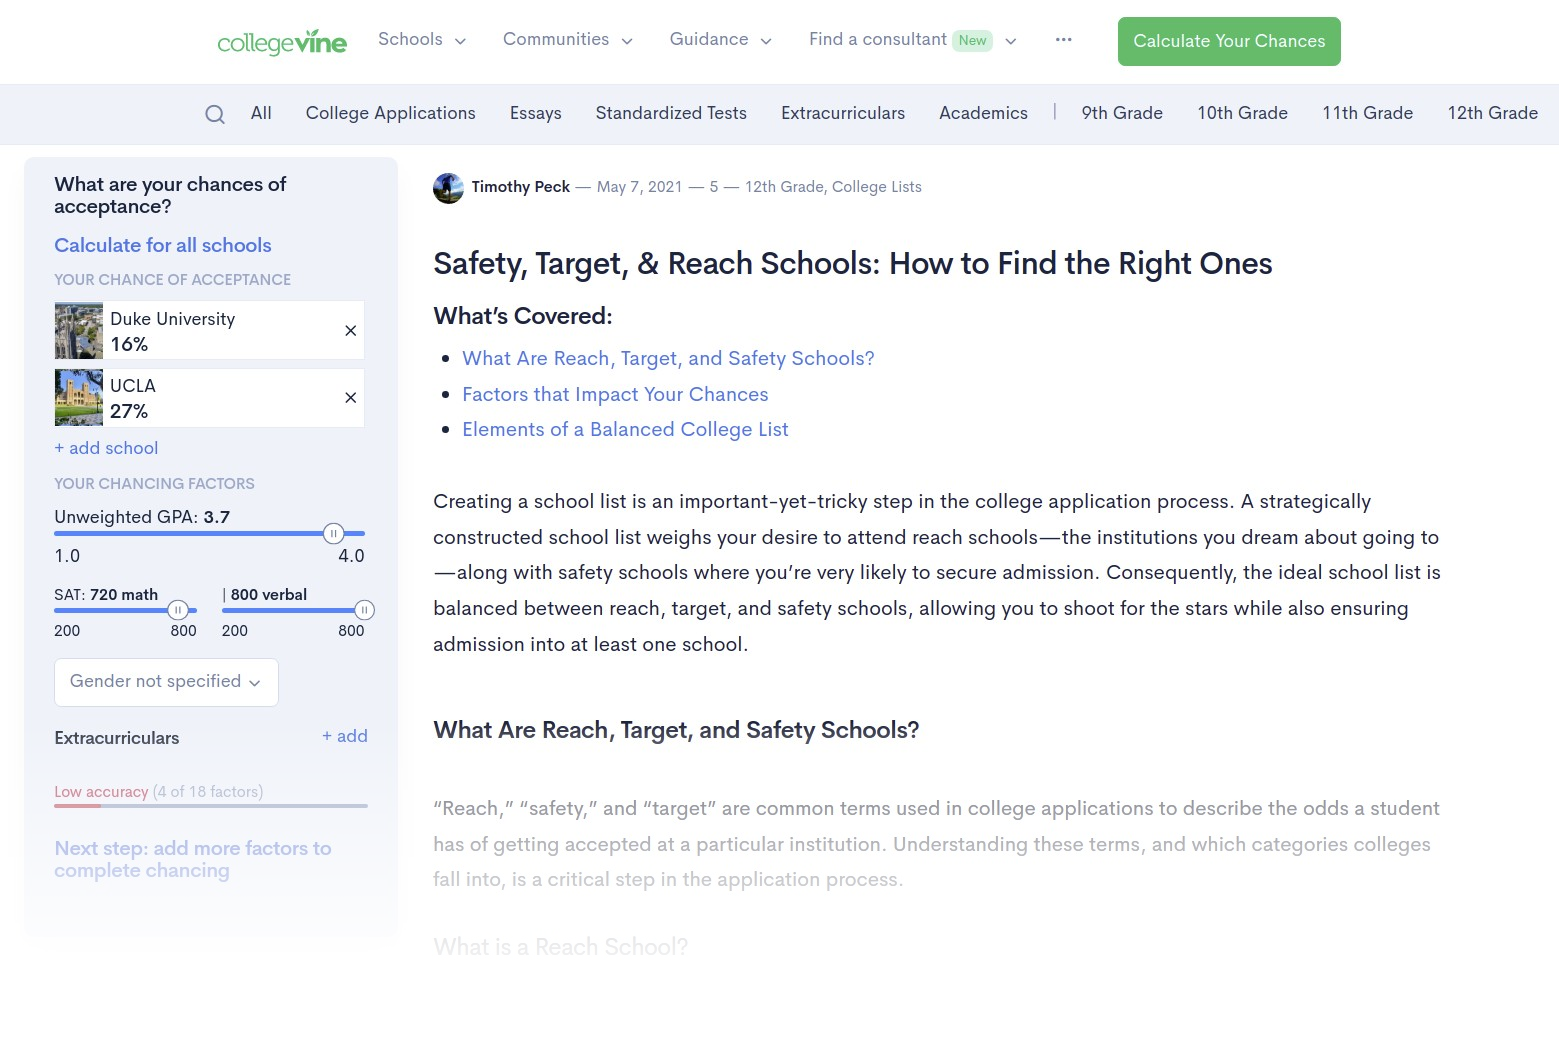
\includegraphics[width=\textwidth]{plots/news-en.png}
\end{center}
\end{frame}
\fi



\begin{frame}[plain]{}
\begin{center}

\includegraphics[width=\textwidth]{plots/news-ko.png}
\end{center}
\end{frame}



\ifen \else
\begin{frame}[plain]{}
\begin{center}
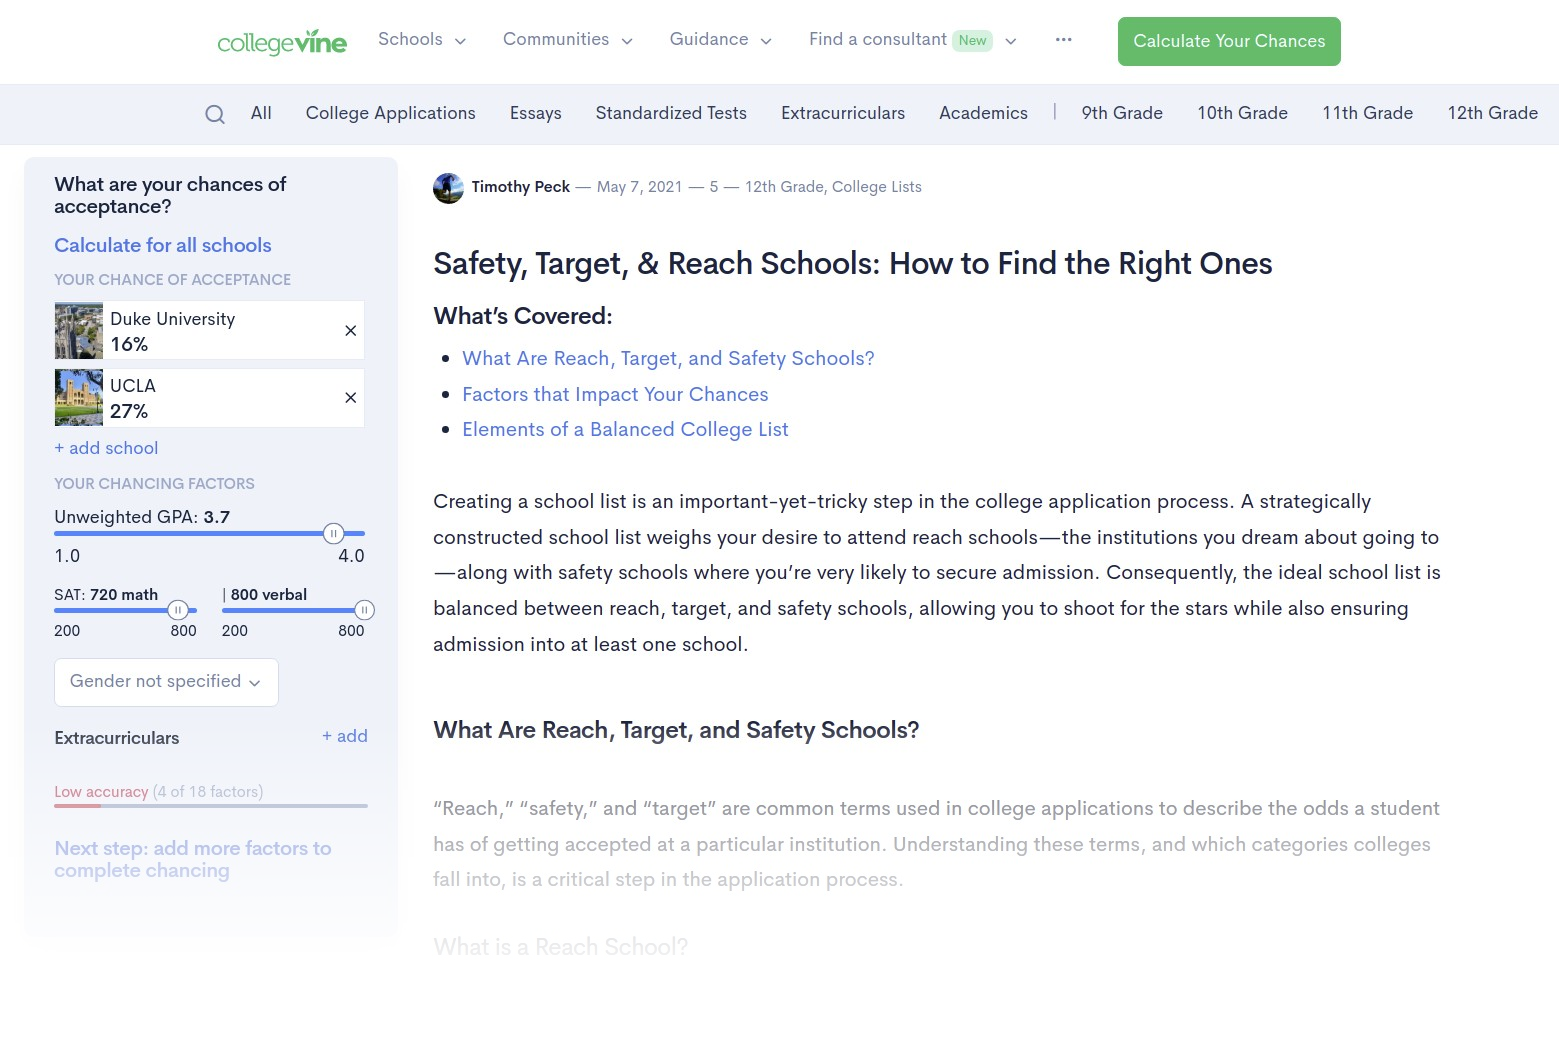
\includegraphics[width=\textwidth]{plots/news-en.png}
\end{center}
\end{frame}
\fi




\begin{frame}[plain]{}
\begin{center}
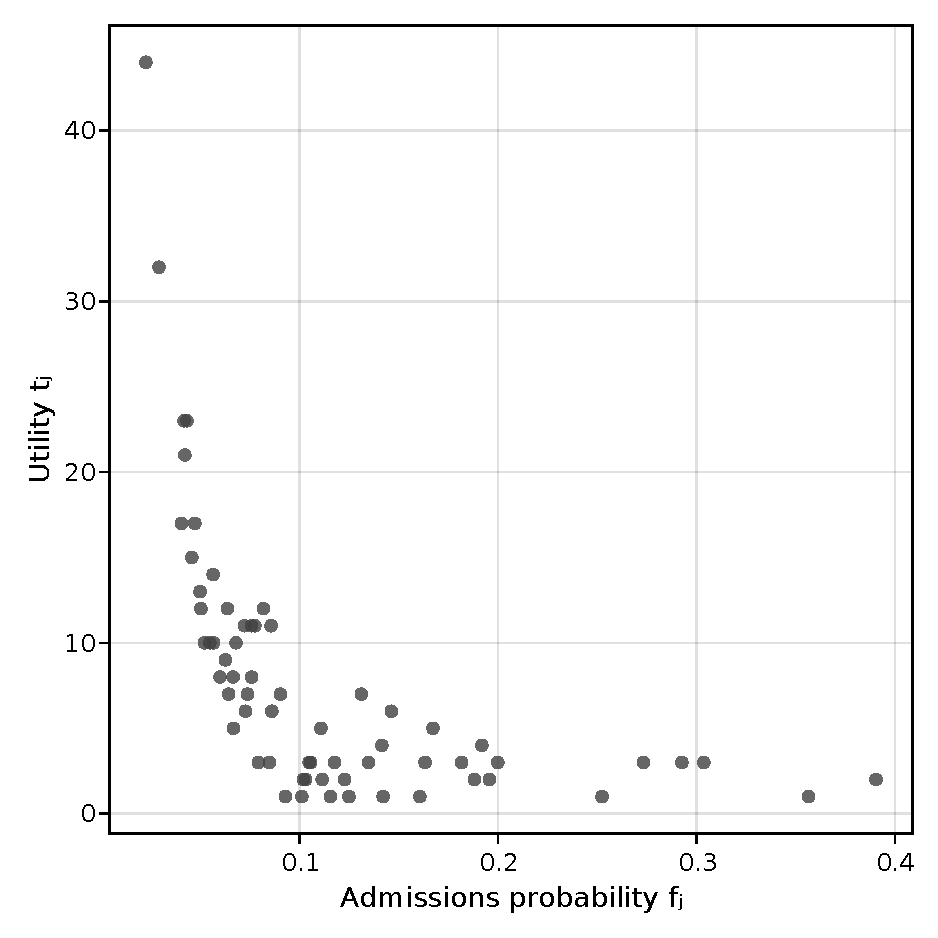
\includegraphics[height=\textheight]{plots/samplemarket.pdf}
\end{center}
\end{frame}





\begin{frame}[plain]{}
\begin{center}
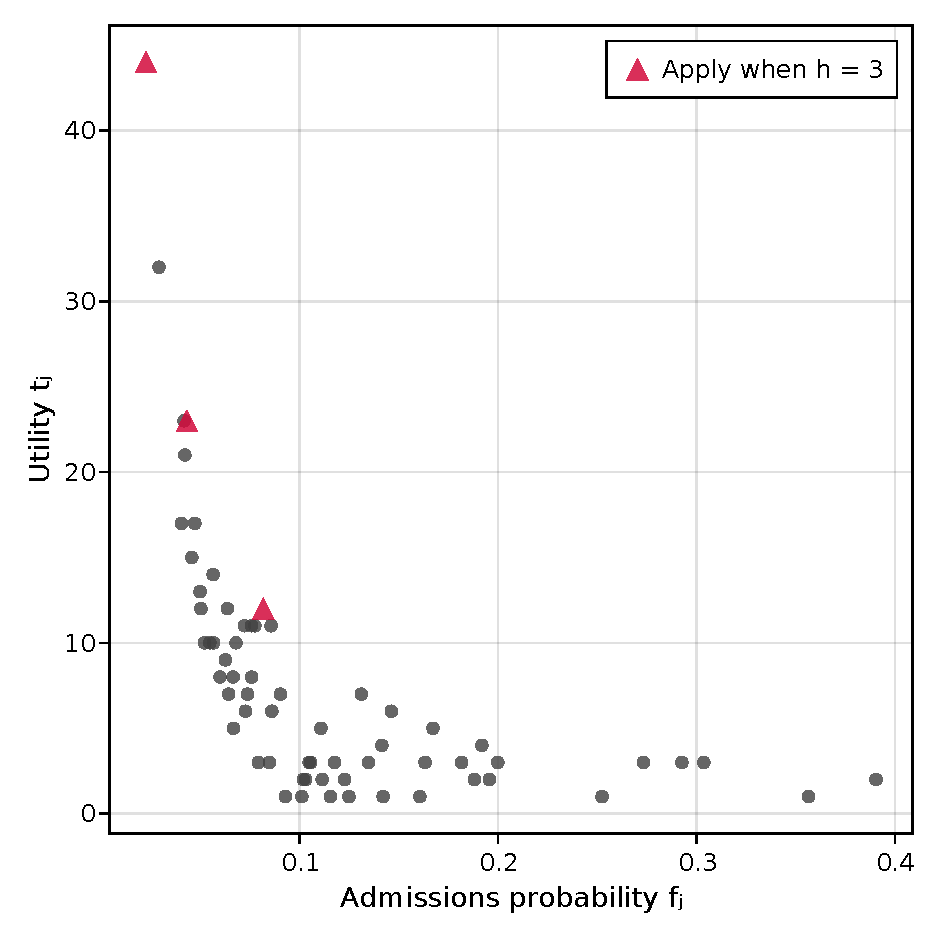
\includegraphics[height=\textheight]{plots/samplemarket-soln.pdf}
\end{center}
\end{frame}








\ifen \section{Alma's problem} \else \section{알마의 문제} \fi

\ifen{
\begin{frame}[plain]
  \vspace{9em}
\begin{center}
~
\begin{beamercolorbox}[wd=.6\textwidth,sep=8pt,center,shadow=false,rounded=true]{section in head/foot}
    \usebeamerfont{title} \insertsectionhead \par%
  \end{beamercolorbox}
~
\end{center}
\end{frame}
}
\else{
\begin{frame}
  \vspace{9em}
\begin{center}
~
\begin{beamercolorbox}[wd=.6\textwidth,sep=8pt,center,shadow=false,rounded=true]{section in head/foot}
    \usebeamerfont{title} \insertsectionhead \par%
  \end{beamercolorbox}
~
\end{center}
\end{frame}
}
\fi

\begin{frame}{\ifen The nestedness property for Alma's problem\else 알마 문제 최적해의 포함 사슬 관계\fi}
\ifen The following theorem says that the solution to Alma's problem is \textbf{nested} in the application limit $h$.
\else 다음 정리는 알마 문제의 최적해가 지원 제한 $h$로 모수화된 \textbf{포함 사슬 관계}를 가진다고 의미한다. \fi
\begin{theorem}[\ifen Nestedness of optimal application portfolios\else 최적 포트폴리오의 포함 사슬 관계\fi] \label{nestedapplication}
\ifen There exists a sequence of portfolios $\{\mathcal{X}_h\}_{h=1}^m$ satisfying the nestedness relation
\else  각 $\mathcal{X}_h$가 지원 제한 $h$에 대한 최적 포트폴리오며 위의 포함 사슬 관계를 만족하는 포트폴리오 수열  $\{\mathcal{X}_h\}_{h=1}^m$가 존재한다.\fi
\begin{equation*}
\mathcal{X}_1 \subset \mathcal{X}_2\subset \dots \subset \mathcal{X}_m
\end{equation*}
\ifen such that each $\mathcal{X}_h$ is an optimal application portfolio when the application limit is $h$.\fi
\end{theorem}

\ifen
This implies the validity of a greedy algorithm that adds schools one at a time, maximizing $v(\mathcal{X})$ at each addition. 

Some additional refinement reduces the computation time to $O(hm)$.
\else
따라서 $v(\mathcal{X})$를 최대화하는 학교를 차례대로 추가하는 탐욕 해법의 타당성이 성립.

이를 좀 더 조정하면 계산 시간을 $O(hm)$으로 절감할 수 있다.
\fi
\end{frame}





\begin{frame}{\ifen Concavity of $v(\mathcal{X}_h)$\else $v(\mathcal{X}_h)$의 오목성\fi}
\ifen The nestedness property implies that Alma's expected utility is a discretely concave function of $h$.
\else 포함 사슬 관계 성질은 알마의 기대 효용이 $h$의 이산 오목 함수임을 의미한다.\fi

\begin{theorem}[\ifen Optimal portfolio valuation concave in $h$\else 최적 포트폴리오 가치의 $h$-오목성\fi] \label{concavityinh}
\ifen For $h = 2 \dots (m-1)$,
\else $h = 2 \dots (m-1)$에 대해,\fi
\begin{equation*}v(\mathcal{X}_h) - v(\mathcal{X}_{h-1}) \geq v(\mathcal{X}_{h+1}) - v(\mathcal{X}_{h}).\end{equation*} 
\end{theorem}

\ifen
Corollary: $v(\mathcal{X}_h)$ is $O(h)$. Paper contains a tight example. 
\else
이의 따름정리로서 $v(\mathcal{X}_h)$가 $O(h)$ 함수가 되며, 논문에서 타이트한 예를 제시. 
\fi
\end{frame}





\begin{frame}{A small example}
\ifen
College data and optimal application portfolios for a fictional market with $m=8$ schools.
\else
$m=8$개의 학교로 이루어진 가상 입학 시장의 대학교 자료와 최적 지원 포트폴리오.
\fi
\begin{center}
\begin{tabular}{r|lcccc}
\ifen\textbf{Index $j$} & \textbf{School $c_j$} & \textbf{Admit prob. $f_j$} & \textbf{Utility $t_j$} & \textbf{Priority} & \textbf{$v(\mathcal{X}_h)$} \\ \hline
\else 
\textbf{지표 $j$} & \textbf{학교 $c_j$} & \textbf{합격 확률 $f_j$} & \textbf{효용 $t_j$}  & \textbf{지원 순위} & \textbf{$v(\mathcal{X}_h)$} \\ \hline  \fi
\\[-.75em]
1 & \ifen Mercury University   \else  수성대  \fi   & 0.39   & 200 & 4   & 230.0   \\
2 & \ifen Venus University     \else  금성대  \fi   & 0.33   & 250 & 2   & 146.7  \\
3 & \ifen Mars University      \else  화성대  \fi   & 0.24   & 300 & 6   & 281.5  \\
4 & \ifen Jupiter University   \else  목성대  \fi   & 0.24   & 350 & 1   & \phantom{0}84.0  \\
5 & \ifen Saturn University    \else  토성대  \fi   & 0.05   & 400 & 7   & 288.8  \\
6 & \ifen Uranus University    \else  천왕성대 \fi   & 0.03   & 450 & 8   & 294.1  \\
7 & \ifen Neptune University   \else  해왕성대 \fi   & 0.10   & 500 & 5   & 257.7  \\
8 & \ifen Pluto College        \else  명왕성대 \fi   & 0.12   & 550 & 3   & 195.1      
\end{tabular}
\end{center}

\ifen 
By the nestedness property, the optimal portfolio when the application limit is $h$ consists of the $h$ schools having priority $h$ or less.

The following slide illustrates the concavity property.
\else
포함 사슬 관계 성질에 따라, 지원 제한이 $h$일 때 최적 포트폴리오는 지원 순위가 $h$ 이하인 $h$개의 학교로 구성된다.

다음 화면에서 나타나는 곡선은 오목성 성질을 보인다.
\fi
\end{frame}


\begin{frame}[plain]
\begin{center}
 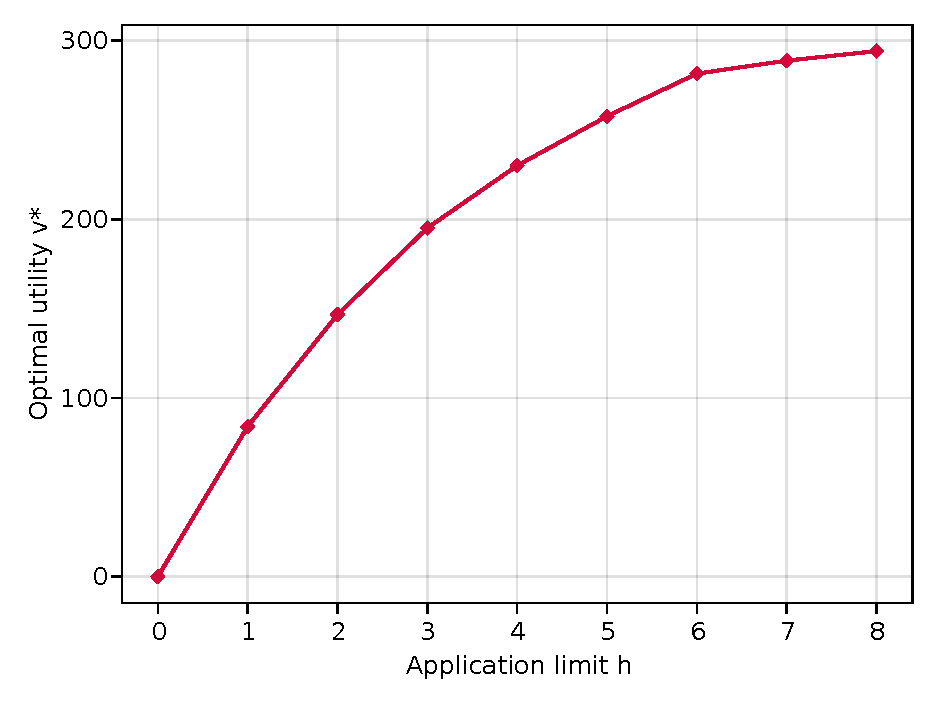
\includegraphics[height=\textheight]{./plots/h_v-example.pdf}
\end{center}
\end{frame}





\section{Ellis's problem}

\ifen{
\begin{frame}[plain]
  \vspace{9em}
\begin{center}
~
\begin{beamercolorbox}[wd=.6\textwidth,sep=8pt,center,shadow=false,rounded=true]{section in head/foot}
    \usebeamerfont{title} \insertsectionhead \par%
  \end{beamercolorbox}
~
\end{center}
\end{frame}
}
\else{
\begin{frame}[plain]
  \vspace{9em}
\begin{center}
~
\begin{beamercolorbox}[wd=.6\textwidth,sep=8pt,center,shadow=false,rounded=true]{section in head/foot}
    \usebeamerfont{title} \insertsectionhead \par%
  \end{beamercolorbox}
~
\end{center}
\end{frame}
}
\fi




\begin{frame}{\ifen Three algorithms for Ellis's problem \else 엘리스의 문제를 위한 3개의 알고리즘\fi}
\ifen {
By setting $f_j = \varepsilon$, we can make $v(\mathcal{X})$ arbitrarily close to a linear function. This means that knapsack reduces to Ellis's problem, and therefore Ellis's problem is NP-complete.

We provide three algorithms for Ellis's problem.
\begin{itemize}
\item \textbf{Branch-and-bound} routine. Theoretically interesting but not very efficient.
\item \textbf{Dynamic program} based on total expeditures. Pseudopolynomial time, namely $O(Hm + m\log m)$, and exact. Very efficient for typical instances in which $g_j$ are small integers.
\item Another dynamic program based on truncated portfolio valuations. Yields a $(1 - \varepsilon)$-optimal solution in $O(m^3 /\varepsilon)$-time: \textbf{an FPTAS}.
\end{itemize}
} \else {
$f_j = \varepsilon$으로 넣으면 $v(\mathcal{X})$를 선형 함수에 원하는 만큼 가깝게 만들 수 있다. 배낭 문제가 엘리스의 문제로 변환할 수 있음을 의미하므로 엘리스의 문제는 NP-complete하다.

엘리스 문제를 위해 3가지해법을 제시한다.
\begin{itemize}
\item \textbf{분지한계법}은 이론적으로 흥미롭지만 현실적 효율성이 낮다.
\item 지원 지출액 기반 \textbf{동적 계획}. $O(Hm + m\log m)$인 의사 다항 시간 안에 정확한 해를 출력하며, $g_j$가 작은 정수가 되는 전형적인 인스턴스에 매우 효율적이다.
\item 분수값을 내림한 포트폴리오 가치 기반 다른 동적 계획. $O(m^3 /\varepsilon)$-시간 안에  $(1 - \varepsilon)$-근사 해를 출력하므로 \textbf{FPTAS}.
\end{itemize}

} \fi
\end{frame}





\ifen \section{Ellis's problem: Branch and bound} \else \section{엘리스의 문제: 분지한계법} \fi

\begin{frame}{\ifen Branch-and-bound\else 분지한계법\fi}
\ifen
Our branch-and-bound framework is based on the following integer formulation of Ellis's problem. 
\else
엘리스의 문제는 다음 정수 비선형 계획으로 표현되며 이를 바탕으로 분지한계법을 만든다. 
\fi
\begin{problem}[\ifen Integer NLP for Ellis's problem\else 엘리스의 문제를 위한 비선형 정수 계획\fi]% \label{integernlp}
\vspace{-1em}
\begin{align*}
\begin{split}
\text{maximize}\quad &  v(x) = \sum_{j=1}^m \Bigl(f_j t_j  x_j \prod_{i > j} (1 - f_{i} x_i) \Bigr)\\
\text{subject to}\quad & \sum_{j=1}^m g_j x_j \leq H, ~~ x_i \in \{0, 1\}^m
\end{split}
\end{align*}
\end{problem}

\ifen
Objective is a nonconvex polynomial of degree $m$ \dots~numerical solvers are hopeless!
\else
목적함수는 $m$차 비오목 다항식 \dots~수리적 솔버는 헛수고!
\fi
\end{frame}






\begin{frame}{\ifen LP relaxation \else 선형 완화 문제\fi}
\ifen 
We use the following LP upper bound.
\else
다음 선형 완화 문제를 활용한다.
\fi
\begin{problem}[\ifen LP relaxation for Ellis's problem\else 엘리스의 문제를 위한 선형 완화 문제\fi] %\label{LPrelaxation}
\vspace{-1em}
\begin{align*}
\begin{split}
\text{maximize}\quad &  v_{\mathrm{LP}}(x) = \sum_{j=1}^m  f_j t_j x_j \\
\text{subject to}\quad & \sum_{j=1}^m g_j x_j \leq H, ~~ x \in [0, 1]^m
\end{split}
\end{align*}
\end{problem}
\ifen
This is a continuous knapsack problem, easy to solve (Dantzig 1957; Balas and Zemel 1980). 

We \textbf{tighten this bound} by recycling a variable-elimination technique from the proof of the nestedness theorem.

A straightforward implementation is OK on small instances ($m \leq 35$). \textbf{Considerable room for improvement} by using better heuristics to select the branch node.
\else
연속 배낭 문제라고 불리며 쉽게 풀 수 있다 (Dantzig 1957; Balas and Zemel 1980). 

포함 사슬 관계의 증명 과정에서 도출한 변수 소거법은 재활용해서 위에 \textbf{상한을 더 타이트하게} 조정한다.

이 기반으로 만든 간단한 알고리즘은 작은 ($m \leq 35$) 인스턴스에 괜찮지만 분지 마디를 선택하는 휴리스틱으로 \textbf{개선할 여지}가 보인다.
\fi
\end{frame}








\ifen \section{Ellis's problem: Expenditures DP} \else \section{엘리스의 문제: 지원 지출액 동적 계획}\fi

\begin{frame}{\ifen Expenditures-based dynamic program\else 지원 지출액 기반 동적 계획\fi}
\ifen Let $V[j,h] $ denote the value of the optimal portfolio that uses only the schools $\{ 1, \dots, j\}$ and costs no more than $h$.
\else $\{ 1, \dots, j\}$에 속한 학교만 사용하면서 지원 지출액이 $h$를 넘지 않은 최적 포트폴리오의 가치를 $V[j, h]$라고 하자.\fi

\ifen Then we can use the following \textbf{Bellman equation} to compute all the $V[j, h]$-values recursively.
\else 그러면 다음과 같은 \textbf{Bellman 식}으로 모든 $V[j, h]$-값은 재귀적으로 계산할 수 있다. \fi
\begin{align*}
V[j, h] = \max\bigl\{ V[j-1, h], (1 - f_j) V[j-1, h-g_j] + f_j t_j \bigr\}
\end{align*}
\ifen
This equation works because the $t_j$-values are indexed in ascending order.

Filling a lookup table with the $V[j, h]$-values therefore costs $O(Hm + m\log m)$, and then computing $\mathcal{X}$ is trivial.

\textbf{Very effective} on typical instances where $g_j$ are small integers.
\else
이 식의 타당성은 학교를 $t_j$-값 순서대로 배열함에 의존.

따라서 $V[j, h]$-값으로 표를 채우는 시간이 $O(Hm + m\log m)$이며 이를 참고하면 $\mathcal{X}$를 쉽게 구할 수 있다.

전형적인 인스턴스에서 $g_j$가 작은 상수이므로 \textbf{매우 효율적인} 해법.
\fi
\end{frame}







\ifen \section{Ellis's problem: Valuations DP} \else \section{엘리스의 문제: 포트폴리오 가치 기반 동적 계획}\fi

\begin{frame}{\ifen Valuation-based dynamic program \else 포트폴리오 가치 기반 동적 계획 \fi}
\ifen 
As with the knapsack problem, Ellis's problem admits a \textbf{complementary dynamic program} that iterates on the value of the cheapest portfolio instead of on the cost of the most valuable portfolio.

We represent approximate portfolio valuations using a \textbf{fixed-point decimal} with a precision of $P$, where $P$ is the number of digits to retain after the decimal point. Let $r[x] =  10^{-P}\lfloor 10^P x \rfloor$ denote the value of $x$ rounded down to its nearest fixed-point representation.

$\bar U = \sum_{j\in \mathcal{C}} f_j t_j$ is an upper bound on the valuation of any portfolio, so the set $\mathcal{V}$ of possible valuations possible in the fixed-point framework is finite:
\else
엘리스의 문제는 배낭 문제와 같이, 가치가 가장 높은 포트폴리오의 비용 대신 비용이 가장 낮은 포트폴리오의 가치를 탐색하는 \textbf{보완적인 동적 계획}이 존재한다. 

포트폴리오의 근사적 가치를 정확도 $P$로 구성된 고정소수점 십진수(fixed-point decimal)로 나타내자. 다, $P$는 소수점 뒤에 등장하는 숫자의 수이다. 이때 $x$를 가장 가까운 고정소수점 십진수로 내림한 것을 $r[x] =  10^{-P}\lfloor 10^P x \rfloor$라고 하자.

임의의 포트폴리오의 가치가 $\bar U = \sum_{j\in \mathcal{C}} f_j t_j$를 넘을 수 없다. 따라서 고정소수점 환경에서 발생할 수 있는 포트폴리오 가치로 이루어진 집합 $\mathcal{V}$는 유한 집합이다.
\fi
\begin{equation*}
\mathcal{V} = \Bigl\{0, 1\times 10^{-P}, 2\times 10^{-P}, \dots, r\bigl[\bar U- 1\times 10^{-P}\bigr], r\bigl[\bar U\bigr]\Bigr\}
\end{equation*}
\ifen Then $|\mathcal{V} | = \bar U \times 10^P + 1$.
\else 그러면 $|\mathcal{V} | = \bar U \times 10^P + 1$이다.\fi

\end{frame}



\begin{frame}{\ifen Recursion relation for valuation DP\else 활용 재귀 관계\fi}
\ifen 
Let $G[j, v]$ denote the application cost of the least expensive portfolio that uses only schools $\{ 1, \dots, j\}$ and has (rounded) valuation at least $v$. We argue that
\else
$\{ 1, \dots, j\}$에 속한 학교만 사용하면 (내림한) 가치가 최소한 $v$의 포트폴리오 중 지원 비용이 최소한 포트폴리오의 지출액을 $G[j, v]$라고 하자. 이때 다음 반복 관계가 성립한다고 주장한다.
\fi
\begin{align*}
G[j, v] &=
\begin{cases}
\infty, \quad & t_j < v \\
\min\bigl\{G[j-1, v], g_j + G[j-1, v - \Delta_j(v)] \bigr\}, \quad & t_j \geq v 
%\begin{cases}
%\min\bigl\{G[j-1, v], g_j + G[j-1, v - \Delta] \bigr\}, \quad &f_j < 1 \\
%\min\bigl\{G[j-1, v], g_j \bigr\}, \quad &f_j = 1 \text{ and } f_j t_j \geq v\\
%G[j-1, v], \quad &f_j = 1 \text{ and } f_j t_j < v
\end{cases}\\
\text{where}\qquad
\Delta_j (v) &= 
\begin{cases}
r\left[\frac{f_j}{1 - f_j} (t_j - v)\right], \quad & f_j < 1\\
\infty, &f_j = 1\ifen.\fi
\end{cases} \label{deltajvdef}
\end{align*}

\ifen
Now we can fill a lookup table with the entries of $G[j, v]$ and compute an approximately optimal portfolio. 

In the paper, we show that setting $P \gets \bigl\lceil\log_{10}\left(m^2 / \varepsilon \bar U\right)\bigr\rceil$ guarantees a $(1- \epsilon)$-optimal portfolio, and that this yields a table of size $O(m^3 / \varepsilon)$, meaning that this algorithm is \textbf{an FPTAS}.
\else
이제 $G[j, v]$-값으로 표를 채우면 근사적 최적 포트폴리오를 구할 수 있다.

논문에서 $P \gets \bigl\lceil\log_{10}\left(m^2 / \varepsilon \bar U\right)\bigr\rceil$로 넣으면 $(1- \epsilon)$-근사해가 보장되며, 해당 표의 크기가  $O(m^3 / \varepsilon)$이므로 이 알고리즘은 \textbf{FPTAS}이다.
\fi
\end{frame}

\ifen
\section{Computational results}
\else
\section{계산 실험 결과}
\fi

\ifen{
\begin{frame}[plain]
  \vspace{9em}
\begin{center}
~
\begin{beamercolorbox}[wd=.6\textwidth,sep=8pt,center,shadow=false,rounded=true]{section in head/foot}
    \usebeamerfont{title} \insertsectionhead \par%
  \end{beamercolorbox}
~
\end{center}
\end{frame}
}
\else{
\begin{frame}[plain]
  \vspace{9em}
\begin{center}
~
\begin{beamercolorbox}[wd=.6\textwidth,sep=8pt,center,shadow=false,rounded=true]{section in head/foot}
    \usebeamerfont{title} \insertsectionhead \par%
  \end{beamercolorbox}
~
\end{center}
\end{frame}
}
\fi





\begin{frame}{\ifen Computational experiment: Alma's problem \else 계산 실험: 알마의 문제\fi}
\ifen 
All algorithms implemented and tested in Julia (v1.8.0b1). 

Generate \textbf{synthetic instances} with partial negative correlation between $f_j$ and $t_j$. 
 
50 markets in each cell, time recorded as best of three reps. Table shows mean (std) computation time in ms.

\textbf{Experiment 1:} Alma's problem. Compare two \textbf{data structures} for $\mathcal{C}$. 
\else
모든 알고리즘은 쥴리아 (Julia, v1.8.0b1) 언어로 구현.

$f_j$와 $t_j$가 반비례하는 \textbf{가상 인스턴스}를 생성.

각 칸에서 50개의 시장을 생성하고 최적해를 3번 계산한 것 중에 최소 시간을 기록. 표에서 나타나는 값은 평균 (표준편차) 시간이며 단위는 ms.

\textbf{실험 1:} 알마의 문제. $\mathcal{C}$를 저장하는 자료 구현 2가지 비교. 
\fi
\begin{center}
\scalebox{0.92}{ %
\begin{tabular}{r|r@{~}r|r@{~}r}
\ifen 
 \textbf{\begin{tabular}[r]{@{}r@{}}\\$m$\end{tabular}}& \multicolumn{2}{c|}{\textbf{\begin{tabular}[c]{@{}c@{}}Greedy alg.\\with list\end{tabular}}}  & \multicolumn{2}{c}{\textbf{\begin{tabular}[c]{@{}c@{}}Greedy alg.\\with heap\end{tabular}}}\\ \hline
 \else
 \textbf{\begin{tabular}[r]{@{}r@{}}\\$m$\end{tabular}}& \multicolumn{2}{c|}{\textbf{\begin{tabular}[c]{@{}c@{}}탐욕 알고리즘\\(목록 구현)\end{tabular}}}  & \multicolumn{2}{c}{\textbf{\begin{tabular}[c]{@{}c@{}}탐욕 알고리즘\\(힙 구현)\end{tabular}}}\\ \hline
 \fi
    16 &           0.00 &        (0.00) &           0.01 &        (0.00) \\
    64 &           0.03 &        (0.00) &           0.08 &        (0.02) \\
   256 &           0.15 &        (0.01) &           0.97 &        (0.22) \\
  1024 &           2.31 &        (0.05) &          14.44 &        (1.66) \\
  4096 &          37.85 &        (0.61) &         245.74 &       (17.33) \\
 16384 &         585.75 &        (2.11) &        4728.59 &      (552.25)
\end{tabular}
}
\end{center}
\ifen 
$\argmax$ operation at each iteration made heap an appealing data structure, but because \emph{every} key is updated, the savings aren't worth the cost.
\else 
반복 단계마다 $\argmax$ 연산이 필요하므로 힙 구현에는 매력이 있지만, 그의 모든 원소를 수정해야 하므로 만회하지 않는다.
\fi

\end{frame}




\begin{frame}{\ifen Computational experiment: Ellis's problem\else 계산 실험: 엘리스의 문제\fi}
\ifen 
\textbf{Experiment 2:} Ellis's problem. Compare the two exact algorithms with the FPTAS at two levels of precision. %
\else 
\textbf{실험 2:} 엘리스의 문제. 2개의 정확한 해법 그리고 2개의 정확도로 실행한 FPTAS를 비교.
\fi
\begin{center}
\scalebox{0.92}{ %
\begin{tabular}{r|r@{~}r|r@{~}r|r@{~}r|r@{~}r} %
\ifen %
\textbf{\begin{tabular}[r]{@{}r@{}}$m$\end{tabular}}&\multicolumn{2}{c|}{\textbf{\begin{tabular}[c]{@{}c@{}}Branch \& bound\end{tabular}}}  & \multicolumn{2}{c|}{\textbf{\begin{tabular}[c]{@{}c@{}}App. costs DP\end{tabular}}}  &\multicolumn{2}{c|}{\textbf{\begin{tabular}[c]{@{}c@{}}FPTAS, $\varepsilon= 0.5$\end{tabular}}}  & \multicolumn{2}{c}{\textbf{\begin{tabular}[c]{@{}c@{}}FPTAS, $\varepsilon= 0.05$\end{tabular}}}   \\ \hline
\else
\textbf{\begin{tabular}[r]{@{}r@{}}$m$\end{tabular}}&\multicolumn{2}{c|}{\textbf{\begin{tabular}[c]{@{}c@{}}분지한계법\end{tabular}}}  & \multicolumn{2}{c|}{\textbf{\begin{tabular}[c]{@{}c@{}}지출액 DP\end{tabular}}}  &\multicolumn{2}{c|}{\textbf{\begin{tabular}[c]{@{}c@{}}FPTAS, $\varepsilon= 0.5$\end{tabular}}}  & \multicolumn{2}{c}{\textbf{\begin{tabular}[c]{@{}c@{}}FPTAS, $\varepsilon= 0.05$\end{tabular}}}   \\ \hline
\fi
     8 &          0.04 &       (0.02) &         0.01 &      (0.00) &                0.05 &             (0.01) &                 0.21 &              (0.06) \\
    16 &          0.22 &       (0.11) &         0.07 &      (0.01) &                0.43 &             (0.10) &                 3.15 &              (0.74) \\
    32 &        166.20 &     (422.31) &         0.31 &      (0.05) &                2.38 &             (0.38) &                33.38 &             (11.68) \\
    64 &             — &          (—) &         1.36 &      (0.18) &               15.32 &             (2.77) &               405.73 &            (125.98) \\
   128 &             — &          (—) &         6.52 &      (0.72) &               84.50 &            (22.59) &              2362.19 &           (1095.11) \\
   256 &             — &          (—) &        31.23 &      (1.91) &             1085.60 &          (1186.24) &             22129.92 &           (6588.40)
\end{tabular}
}
\end{center}
\ifen 
\textbf{Costs DP has a pronounced advantage} because $g_j$ are small integers, but this is typical of real instances.

Bottleneck for FPTAS is computer memory rather than time. 
\else
실험 데이터에서 $g_j$가 작은 정수이므로 \textbf{지원 지출액 기반 동적 계획은 상당한 우위}를 발휘.

FPTAS의 병목 요소는 계산 시간이 아니라 메모리 소모량.
\fi

\end{frame}






\section{\ifen Conclusion\else 결론\fi}

\ifen{
\begin{frame}[plain]
  \vspace{9em}
\begin{center}
~
\begin{beamercolorbox}[wd=.6\textwidth,sep=8pt,center,shadow=false,rounded=true]{section in head/foot}
    \usebeamerfont{title} \insertsectionhead \par%
  \end{beamercolorbox}
~
\end{center}
\end{frame}
}
\else{
\begin{frame}[plain]
  \vspace{9em}
\begin{center}
~
\begin{beamercolorbox}[wd=.6\textwidth,sep=8pt,center,shadow=false,rounded=true]{section in head/foot}
    \usebeamerfont{title} \insertsectionhead \par%
  \end{beamercolorbox}
~
\end{center}
\end{frame}
}
\fi






\begin{frame}{\ifen Conclusion\else 결론\fi}
\ifen {
Maximax form, integrality constraint make college application an \textbf{interesting optimization problem} with immediate \textbf{practical application}.

Our study \textbf{extends previous work} on greedy approximation algorithms and nestedness properties of optima (Fisher et al. 1978; Rozanov and Tamir 2020).% Portfolio valuation function is similar to a \emph{convex ordered median function} under the change of variables $y_j = t_j x_j$. 

Nestedness property for Alma's problem and the NP-completeness of the general problem is \textbf{analogous to knapsack}.

\textbf{Possible extensions} of our model:
\begin{itemize}
\item Explicit treatment of risk aversion as in the classic Markowitz (1952) model.
\item Diversification constraints like Korea's application fields.
\item Reduce memory usage of dynamic programs. 
\end{itemize}
} \else {
Maximax 형태와 정수 조건 때문에 대학 지원 전략은 \textbf{흥미로운 최적화 문제}이며 또한 \textbf{실용 가치}가 있다.

본 연수는 탐욕 근사 해법과 최적해의 포함 사슬 관계를 살펴본 \textbf{선행 연구의 확장}으로 볼 수 있다 (Fisher et al. 1978; Rozanov and Tamir 2020).% 결정 변수를 $y_j = t_j x_j$로 변환하면 포트폴리오 가치 함수는 convex ordered median 함수와 닮는다.

알마 문제의 포함 사슬 관계 성질과 일반 문제의 NP-completeness는 \textbf{배낭 문제와 유사한} 결과.

\textbf{향후 연구 방향:}
\begin{itemize}
\item 고전적 Markowitz (1952)자산배분 모형처럼, 위험 회피를 명시적으로 다루는 새로운 목적함수.
\item 한국 입학 과정의 가나다군과 같은 다각화 제약 조건.
\item 동적 계획의 메모리 소모량 절감. 
\end{itemize}
} \fi
\end{frame}
















\begin{frame}[allowframebreaks]{\ifen References \else 참고 문헌 \fi}
\parskip 0em
\leftskip 2em
\parindent -2em
Balas, Egon and Eitan Zemel. 1980. ``An Algorithm for Large Zero-One Knapsack Problems.'' \emph{Operations Research} 28 (5): 1130--54. \url{https://doi.org/10.1287/opre.28.5.1130}. 

Dantzig, George B. 1957. ``Discrete-Variable Extremum Problems.'' \emph{Operations Research} 5 (2): 266--88.

Fisher, Marshall, George Nemhauser, and Laurence Wolsey. 1978. ``An analysis of approximations for maximizing submodular set functions—I.'' \emph{Mathematical Programming} 14: 265--94. 

Fu, Chao. 2014. ``Equilibrium Tuition, Applications, Admissions, and Enrollment in the College Market.'' \emph{Journal of Political Economy} 122 (2): 225--81. \url{https://doi.org/10.1086/675503}. 

Markowitz, Harry. 1952. ``Portfolio Selection.'' \emph{The Journal of Finance} 7 (1): 77--91. \url{https://www.jstor.org/stable/2975974}.

\framebreak

Rozanov, Mark and Arie Tamir. 2020. ``The nestedness property of the convex ordered median location problem on a tree.'' \emph{Discrete Optimization} 36: 100581. \url{https://doi.org/10.1016/j.disopt.2020.100581}.

Sklarow, Mark. 2018. \emph{State of the Profession 2018: The 10 Trends Reshaping Independent Educational Consulting.} Technical report, Independent Educational Consultants Association. \url{https://www.iecaonline.com/wp-content/uploads/2020/02/IECA-Current-Trends-2018.pdf}.

\end{frame}












\begin{frame}[plain]
\begin{center}
 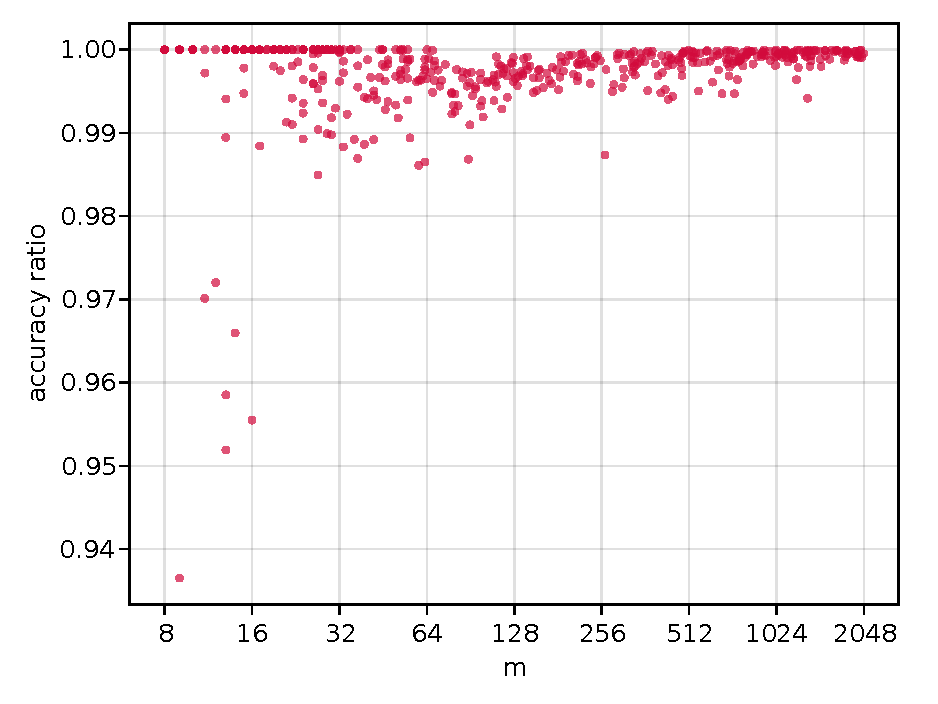
\includegraphics[height=\textheight]{./plots/accuracy_simulatedannealing.pdf}
\end{center}
\end{frame}





\begin{frame}{Abstract}
This paper considers the maximization of the expected maximum value of a portfolio of random variables subject to a budget constraint. We refer to this as the optimal college application problem. When each variable's cost, or each college's application fee, is identical, we show that the optimal portfolios are nested in the budget constraint, yielding an exact polynomial-time algorithm. When colleges differ in their application fees, we show that the problem is NP-complete. We provide four algorithms for this more general setup: a branch-and-bound routine, a dynamic program that produces an exact solution in pseudopolynomial time, a different dynamic program that yields a fully polynomial-time approximation scheme, and a simulated-annealing heuristic. Numerical experiments demonstrate the algorithms' accuracy and efficiency. 
\end{frame}




\ifen \else
\begin{frame}{요약}
본 논문은 다수의 확률 변수로 구성된 포트폴리오의 기대 최댓값을 예산 조건 하에서 최대화하는 문제를 고려한다. 이를 대학 지원 최적화 문제라고 부른다. 각 확률 변수의 비용, 즉 각 대학의 지원 비용이 동일한 경우, 최적 포트폴리오는 예산 제약식으로 결정된 포함 사슬 관계 성질을 가짐을 보이고 이를 바탕으로 다항 시간 해법을 제시한다. 대학의 지원 비용이 서로 다른 경우, 문제가 NP-complete함을 증명한다. 일반적인 문제를 위해 4가지 해법을 제시한다. 분지한계 기반 해법, 의사 다항 시간 안에 정확한 해를 출력하는 동적 계획 해법, 다른 동적 계획 기반으로 완전 다항 시간 근사 해법(fully polynomial-time approximation scheme), 그리고 모의 담금질(simulated annealing)을 이용한 휴리스틱 해법. 
% 첫째는 분지한계 기반 해법이다. 둘째는 의사 다항 시간 안에 정확한 해를 출력하는 동적 계획 해법이다. 마지막으로 다른 동적 계획 기반으로 완전 다항 시간 근사 해법(fully polynomial-time approximation scheme)을 도출한다.
수리적 실험을 통하여 알고리즘의 정확도와 효율성을 보인다.
\end{frame}

\fi








